\documentclass[
]{jss}

%% recommended packages
\usepackage{orcidlink,thumbpdf,lmodern}

\usepackage[utf8]{inputenc}

\author{
Piotr Chlebicki~\orcidlink{0009-0006-4867-7434}\\Stockholm
University \And Maciej
Beręsewicz~\orcidlink{0000-0002-8281-4301}\\Poznań University of
Economics and Business\\
Statistical Office in Poznań
}
\title{\pkg{singleRcapture}: An \proglang{R} Package for Single-Source
Capture-Recapture Models}

\Plainauthor{Piotr Chlebicki, Maciej Beręsewicz}
\Plaintitle{singleRcapture: An R Package for Single-Source
Capture-Recapture Models}
\Shorttitle{\pkg{singleRcapture}: Single-Source Capture-Recapture
Models}


\Abstract{
The estimation of population size represents a significant challenge
within the domains of official statistics, social sciences, and natural
sciences. In such situations capture-recapture methods can be applied,
which can be classified according to the number of sources utilized,
particularly whether a single or multiple sources are employed. This
paper focuses on the first group of methods and introduces the package
\pkg{singleRcapture}. The package implements state-of-the-art
single-source capture-recapture models (e.g.~zero-truncated one-inflated
regression), new developments proposed by the authors, and provides a
user-friendly application programming interface (API). The package is
self-contained, providing point estimates and their variance, as well as
implementing several bootstrap variance estimators or diagnostics to
assess quality and conduct sensitivity analysis. It is intended for
users interested in estimating the size of populations, particularly
those that are difficult to reach or measure, for which information is
available from only one source and dual/multiple system estimation is
not applicable.
}

\Keywords{population size estimation, hidden populations, truncated
distributuons, count regression models, \proglang{R}}
\Plainkeywords{population size estimation, hidden populations, truncated
distributuons, count regression models, R}

%% publication information
%% \Volume{50}
%% \Issue{9}
%% \Month{June}
%% \Year{2012}
%% \Submitdate{}
%% \Acceptdate{2012-06-04}

\Address{
    Piotr Chlebicki\\
    Stockholm University\\
    Matematiska institutionen\\
Albano hus 1\\
106 91 Stockholm, Sweden\\
  E-mail: \email{piotr.chlebicki@math.su.se}\\
  URL: \url{https://github.com/Kertoo},
\url{https://www.su.se/profiles/pich3772}\\~\\
      Maciej Beręsewicz\\
    Poznań University of Economics and Business\\
Statistical Office in Poznań\\
    Poznań University of Economics and Business\\
Department of Statistics\\
Institute of Informatics and Quantitative Economics\\
Al. Niepodległosci 10\\
61-875 Poznań, Poland\\
\strut \\
Statistical Office in Poznań\\
ul. Wojska Polskiego 27/29\\
60-624 Poznań, Poland\\
  E-mail: \email{maciej.beresewicz@ue.poznan.pl}\\
  
  }


% tightlist command for lists without linebreak
\providecommand{\tightlist}{%
  \setlength{\itemsep}{0pt}\setlength{\parskip}{0pt}}




\usepackage{amsmath, amsthm, amssymb} \usepackage{calc, ragged2e} \usepackage[ruled]{algorithm2e}

\DeclareMathAlphabet{\mathmybb}{U}{bbold}{m}{n}
\newcommand{\1}{\mathcal{I}} \newcommand{\bZero}{\boldsymbol{0}}
\newcommand{\bx}{\boldsymbol{x}} \newcommand{\bX}{\boldsymbol{X}}
\newcommand{\bbeta}{\boldsymbol{\beta}}
\newcommand{\boeta}{\boldsymbol{\eta}} \newcommand{\bW}{\boldsymbol{W}}
\newcommand{\bo}{\boldsymbol{o}}

\begin{document}



\section{Introduction}\label{sec-introduction}

Population size estimation is a methodological approach employed across
multiple scientific disciplines, serving as a basis for research, policy
formulation, and decision-making processes \citep{bohning2018capture}.
In the field of statistics, particularly official statistics, precise
population estimates are essential for developing robust economic
models, optimizing resource allocation, and informing evidence-based
policy formulation \citep[cf.][]{baffour-awuah2009}. Social scientists
utilize advanced population estimation techniques to investigate
\emph{hard-to-reach} populations, such as homeless individuals or
illicit drug users, thereby addressing the inherent limitations of
conventional census methodologies. These techniques are crucial for
obtaining accurate data on populations that are typically
under-represented or difficult to access through traditional sampling
methods \citep{vincent2022estimating}. In ecology and epidemiology,
researchers focus on estimating the size of specific species or
disease-affected populations within defined geographical regions, which
is vital for conservation efforts, ecosystem management, and public
health interventions.

Population size estimation can be approached through various
methodologies, each with distinct advantages and limitations.
Traditional approaches include full enumeration (e.g.~census operations)
and comprehensive sample surveys, which, while providing detailed data,
are often resource-intensive and may result in delayed estimates,
particularly for human populations. Alternative methods leverage
existing data sources, such as administrative registers or carefully
designed small-scale studies in wildlife research or census coverage
surveys \citep{wolter1986some, zhang2019note}. Application of these
sources often comes with statistical methods, known as
\emph{capture-recapture} or \emph{multiple system estimation}, that
utilizes data from multiple enumerations of the same population
\citep[cf.][]{dunne2024system}. This can be implemented using a single
source with repeated observations, two, or multiple sources.

In this paper we focus methods that utilize a single data source with
multiple enumerations of the same units \citep[cf.][]{ztpoisson}. In
human population studies, such data might be derived from police
records, health system databases, or border control logs, while for
non-human populations, veterinary records or specialized field data
serve as analogous sources. These methods are often applied for
hard-to-reach or hidden population where standard sampling methods may
be inappropriate because of the costs or problems with identification of
members of these populations.

While methods for two or more sources are implemented in various
open-source software, for instance \pkg{Rcapture}
\citep{baillargeon2007rcapture}, \pkg{marked} \citep{laake2013marked} or
\pkg{VGAM} \citep{yee2015vgam} the single-source capture-recapture
(SSCR) methods are less available being only partially implemented in
existing \proglang{R} packages. The goal of the paper is to introduce
the \pkg{singleRcapture} and \pkg{singleRcaptureExtra} packages which by
implementing \emph{state-of-the-art} methods in SSCR and providing user
friendly API which mimics existing \proglang{R} functions (e.g.,
\texttt{glm}) attempt to bridge this aforementioned gap. In the next
subsection we describe the available \proglang{R} packages that could be
used for estimating population size based on SSCR methods.

\subsection{Software for capture-recapture for single and multiple
sources}\label{sec-software}

Majority of SSCR methods assume zero-truncated distributions or their
extensions (e.g., inclusion of one-inflation). The \pkg{countreg}
\citep{countreg}, \pkg{VGAM} \citep{VGAM-main} or \pkg{distributions3}
\citep{distributions3} implement some of those truncated distributions
and the most general distributions such as Generally Altered, Inflated,
Truncated and Deflated (GAITD) can be found in the \pkg{VGAM}. However,
estimation of parameters of a given truncated (and possibly inflated)
distribution is just a first step (similarly as in log-linear models in
capture-recapture with two sources) and to best of our knowledge there
is no open-source software that allows to estimate population size based
on SSCR method, including variance estimator or diagnostics.

Therefore, the goal of the \pkg{singleRcapture} is \proglang{R} language
is to bridge this gap to provide scientists and other practitioners a
tool for estimation of population size based on SSCR methods. The
package implements state-of-the-art methods as recently described by
\citet{bohning2018capture} or \citet{bohning2024one} and its extensions
(e.g., inclusion of covariates, different treatment of one-inflation)
that we will cover in detail in Section 1. The package implements
variance estimation based on various methods, allows for implementing
custom models as well as diagnostics plots (e.g.~rootograms) with
parameters estimated using a modified IRLS algorithm implemented by us
to for estimation stability. Furthermore, as many \proglang{R} users are
familiar with \pkg{countreg} or \pkg{VGAM} we have implemented a
lightweight extension \pkg{singleRcaptureExtra}, available through
Github (\url{https://github.com/ncn-foreigners/singleRcaptureExtra}),
that allows for integration of \pkg{singleRcapture} with those packages.

The remaining part of the paper is as follows. In Section
\ref{sec-theory} a brief description of the theoretical background is
given and information on the fitting methods, the available methods and
variance estimation is presented. In Section \ref{sec-main} the main
functionalities of the package are introduced. Section \ref{sec-study}
provides a case study along with assessment of results, diagnostics and
estimation of specific sub-populations. Section \ref{sec-methods} covers
classes and \code{S3methods} implemented in the package. Section
\ref{sec-vgam} covers integration with \pkg{countreg} and \pkg{VGAM}
packages through \pkg{singleRcaptureExtra} package. The paper ends with
conclusions and an appendix that shows how to a implement custom model
and how one can use the \code{estimatePopsizeFit} which is faster than
the main function but only estimates regression, which could be of
interest to users interested in using any new bootstrap methods not
programmed in the package (see Appendix \ref{sec-estimatePopsizeFit}).

\section{Theoretical background}\label{sec-theory}

\subsection{How do we estimate population size with a single
register?}\label{how-do-we-estimate-population-size-with-a-single-register}

Let \(Y_{k}\) represent the number of times \(k\)-th unit was observed
in a register. Clearly, we only observe \(k:Y_{k}>0\) and we do not know
how many units are missed (i.e.~\(Y_{k}=0\)) and to find the population
size denoted by \(N\) we need to estimate it. In general, we assume that
conditional distribution of \(Y_{k}\) given a vector of covariates
\(\boldsymbol{x}_{k}\) follows some version of zero-truncated count data
distribution (and its extensions). Knowing the parameters of the
distribution we may estimate the population size using Horowitz-Thompson
type estimator given by:

\begin{equation}
\hat{N}=
\sum_{k=1}^{N}\frac{I_{k}}{\mathbb{P}[Y_{k}>0|\boldsymbol{X}_{k}]}=
\sum_{k=1}^{N_{obs}}\frac{1}{\mathbb{P}[Y_{k}>0|\boldsymbol{X}_{k}]},
\label{eq-ht-estimator}
\end{equation}

where \(I_{k}:=\mathcal{I}_{\mathbb{N}}(Y_{k})\) and \(\mathcal{I}\) is
the indicator function, and maximum likelihood estimate of \(N\) is
obtained after substituting regression parameters \(\boldsymbol{\beta}\)
for \(\mathbb{P}[Y_{k}>0|\boldsymbol{x}_{k}]\) into
\eqref{eq-ht-estimator}.

The basic SSCR assumes independence between counts which may be rather
naive as the first capture may significantly influence the behaviour of
a given unit or limit possibilities of further captures (e.g.~due to
incarceration). To solve these issues, \citet{godwin2017estimation} and
\citet{ztoi-oizt-poisson} introduced one-inflated distributions that
explicitly model probability of the singletons by giving additional mass
\(\omega\) for singletons denoted as \(\mathcal{I}_{\{1\}}(y)\)
\citep[cf.][]{bohning2024one}

\begin{equation*}
  \mathbb{P}^{\ast}[Y=y|Y>0] =
  \omega\mathcal{I}_{\{1\}}(y)+(1-\omega)\mathbb{P}[Y=y|Y>0].
\end{equation*}

The analytic variance estimation is then done by computing two parts of
the decomposition due to the law of total variance given by:

\begin{equation}\label{eq-law_of_total_variance_decomposition}
  \text{var}[\hat{N}] = \mathbb{E}\left[\text{var}
  \left[\hat{N}|I_{1},\dots,I_{n}\right]\right] + 
  \text{var}\left[\mathbb{E}[\hat{N}|I_{1},\dots,I_{n}]\right],
\end{equation}

where the first part can be estimated using the multivariate \(\delta\)
method given by:

\begin{equation*}
  \mathbb{E}\left[\text{var} \left[\hat{N}|I_{1},\dots,I_{n}\right]\right] =
  \left.\left(\frac{\partial(N|I_1,\dots,I_N)}{\partial\boldsymbol{\beta}}\right)^\top
  \text{cov}\left[\hat{\boldsymbol{\beta}}\right]
  \left(\frac{\partial(N|I_1,\dots,I_N)}{\partial\boldsymbol{\beta}}\right)
  \right|_{\boldsymbol{\beta}=\hat{\boldsymbol{\beta}}},
\end{equation*}

while the second part of the decomposition in
\eqref{eq-law_of_total_variance_decomposition} is under the assumption
of independence of \(I_{k}\)'s and after some omitted simplifications is
optimally estimated by:

\begin{equation*}
  \text{var}\left(\mathbb{E}(\hat{N}|I_{1},\dots,I_{n})\right) =
  \text{var}\left(\sum_{k=1}^{N}\frac{I_{k}}{\mathbb{P}(Y_{k}>0)}\right)
  \approx\sum_{k=1}^{N_{obs}}\frac{1-\mathbb{P}(Y_{k}>0)}{\mathbb{P}(Y_{k}>0)^{2}},
\end{equation*}

which forms the basis for the interval estimation. Confidence intervals
are usually constructed under the assumption of (asymptotic) normality
of \(\hat{N}\) or asymptotic normality of \(\ln(\hat{N}-N)\) (or log
normality of \(\hat{N}\)). The latter of which is an attempt to address
a common criticism of student type confidence intervals in SSCR, that is
a possibly skewed distribution of \(\hat{N}\), and results in the
\(1-\alpha\) confidence interval given by:

\begin{equation*}
  \left(N_{obs}+\frac{\hat{N}-N_{obs}}{\xi},N_{obs} +
  \left(\hat{N}-N_{obs}\right)\xi\right),
\end{equation*}

where:

\begin{equation*}
  \xi = \exp\left(z\left(1-\frac{\alpha}{2}\right)
  \sqrt{\ln\left(1+\frac{\widehat{\text{Var}}(\hat{N})}{\left(\hat{N}-N_{obs}\right)^{2}}\right)}\right).
\end{equation*}

and where \(z\) is the quatile function of the standard normal
distribution. The estimator \(\hat{N}\) is best interpreted as being an
estimator for the total number of \underline{observable} units in the
population since we have no means of estimating the number of units in
the population for which the probability of being included in the data
is \(0\) \citep[cf.][]{ztpoisson}.

\subsection{Available models}\label{available-models}

The full list of implemented models in \pkg{singleRcapture} along with
the expressions for probability density functions and point estimates
can be found in the collective help file for all family functions:

\begin{CodeChunk}
\begin{CodeInput}
R> ?ztpoisson
\end{CodeInput}
\end{CodeChunk}

For the sake of simplicity we limit ourselves to just listing the family
functions:

\begin{itemize}
    \item Generalized Chao's \citep{chao1987estimating} and Zelterman's \citep{zelterman1988robust} estimators via logistic regression on variable $Z$ defined as $Z=1$ if $Y=2$ and $Z=0$ if $Y=1$ with $Z\sim b(p)$ where $b(\cdot)$ is the Bernoulli distribution and $p$ can be modeled for each unit $k$ by $\text{logit}(p_k)=\ln(\lambda_k/2)$ with Poisson parameter $\lambda_k=\boldsymbol{x}_{k}\boldsymbol{\beta}$ (for covariate extension see \cite{chao-generalization} and \cite{zelterman}):
    \begin{align}
        \hat{N} &= N_{obs}+
        \sum_{k=1}^{\boldsymbol{f}_{1}+\boldsymbol{f}_{2}}
        \left(2\exp\left(\boldsymbol{x}_{k}\hat{\boldsymbol{\beta}}\right)+
        2\exp\left(2\boldsymbol{x}_{k}\hat{\boldsymbol{\beta}}\right)\right)^{-1},
        \tag{\text{Chao's estimator}}\\
        \hat{N}&=\sum_{k=1}^{N_{obs}}
        \left(1-\exp\left(-2\exp\left(\boldsymbol{x}_{k}\hat{\boldsymbol{\beta}}\right)\right)\right)^{-1}.
        \tag{\text{Zelterman's estimator}}
    \end{align}
    \item Zero-truncated (\code{zt}$^\ast$) and zero-one-truncated (\code{zot}$^\ast$) Poisson \citep[cf. ][]{zotmodels}, geometric, NB type II (NB2) regression where the non-truncated distribution is parameterized as:
    \begin{equation*}
        \mathbb{P}[Y=y|\lambda,\alpha] = \frac{\Gamma\left(y+\alpha^{-1}\right)}{\Gamma\left(\alpha^{-1}\right)y!}
        \left(\frac{\alpha^{-1}}{\alpha^{-1}+\lambda}\right)^{\alpha^{-1}}
        \left(\frac{\lambda}{\lambda + \alpha^{-1}}\right)^{y}.
    \end{equation*}
    \item Zero-truncated one-inflated (\code{ztoi}$^\ast$) modifications distributions where the new probability $\mathbb{P}^{\ast}$ measure is defined in terms of count data measure $\mathbb{P}$ with support on $\mathbb{N}\cup\{0\}$ as:
    \begin{equation*}
    \mathbb{P}^{\ast}[Y=y]=
    \begin{cases}
    \mathbb{P}[Y=0] & y=0, \\
    \omega\left(1-\mathbb{P}[Y=0]\right)+(1-\omega)\mathbb{P}[Y=1] & y=1, \\
    (1-\omega)\mathbb{P}[Y=y] & y>1,
    \end{cases}
    \end{equation*}
    \begin{equation*}
        \mathbb{P}^{\ast}[Y=y|Y>0]=\omega\mathcal{I}_{\{1\}}(y)+(1-\omega)\mathbb{P}[Y=y|Y>0].
    \end{equation*}
    \item One-inflated zero-truncated (\code{oizt}$^\ast$) modifications distributions where the new probability $\mathbb{P}^{\ast}$ measure is defined as:
    \begin{equation*}
        \mathbb{P}^{\ast}[Y=y] = \omega \mathcal{I}_{\{1\}}(y)+(1-\omega)\mathbb{P}[Y=y],
    \end{equation*}
    \begin{equation*}
        \mathbb{P}^{\ast}[Y=y|Y>0] = 
        \omega\frac{\mathcal{I}_{\{1\}}(y)}{1-(1-\omega)\mathbb{P}[Y=0]}+
        (1-\omega)\frac{\mathbb{P}[Y=y]}{1-(1-\omega)\mathbb{P}[Y=0]}.
    \end{equation*}
    Note that \code{ztoi}$^\ast$ and \code{oizt}$^\ast$ distributions are equivalent as shown by \cite{bohning2023equivalence} but population size estimators are different.
\end{itemize}

In addition, we have provided two new approaches that allow modelling
singletons in a similar way as in Hurdle models. In particular we have
proposed the following:

\begin{itemize}
    \item Zero-truncated Hurdle model (\code{ztHurdle}$^\ast$) for Poisson, geometric and NB2 is defined as:
    \begin{equation*}
        \mathbb{P}^{\ast}[Y=y]=\begin{cases}
        \frac{\mathbb{P}[Y=0]}{1-\mathbb{P}[Y=1]} & y=0, \\
        \pi(1-\mathbb{P}[Y=1]) & y=1, \\
        (1-\pi) \frac{\mathbb{P}[Y=y]}{1-\mathbb{P}[Y=1]} & y>1,
        \end{cases}
    \end{equation*}
    \begin{equation*}
        \mathbb{P}^{\ast}[Y=y|Y>0]=\pi\mathcal{I}_{\{1\}}(y)+
        (1-\pi)\mathcal{I}_{\mathbb{N}\setminus\{1\}}(y)\frac{\mathbb{P}[Y=y]}{1-\mathbb{P}[Y=0]-\mathbb{P}[Y=1]}.
    \end{equation*}
    \item The Hurdle zero-truncated (\code{Hurdlezt}$^\ast$) for Poisson, geometric and NB2 is defined as:
    \begin{align*}
        \mathbb{P}^{\ast}[Y=y]&=\begin{cases}
        \pi & y=1, \\
        (1-\pi) \frac{\mathbb{P}[Y=y]}{1-\mathbb{P}[Y=1]} & y\neq1,
        \end{cases}\\
        \mathbb{P}^{\ast}[Y=y|Y>0]&=\begin{cases}
            \pi\frac{1-\mathbb{P}[Y=1]}{1-\mathbb{P}[Y=0]-\mathbb{P}[Y=1]} & y=1,\\
            (1-\pi)\frac{\mathbb{P}[Y=y]}{1-\mathbb{P}[Y=0]-\mathbb{P}[Y=1]} & y>1.
        \end{cases}
    \end{align*}
\end{itemize}

The approaches presented above differ in terms of assumptions,
computational complexity, or how they treat heterogeneity of captures
and singletons. For instance, the dispersion parameter \(\alpha\) in the
NB2 type models is often interpreted as measuring the
\textit{severeness} of unobserved heterogeneity in the underlying
poisson process \citep[cf.][]{ztnegbin}. When using any truncated NB
model the hope is that due to the class of models considered the
consistency is not lost despite the lack of information.

While not discussed in the literature yet the interpretation of
heterogeneous \(\alpha\) across the population (specified in
\code{controlModel}) would be that the unobserved heterogeneity affects
the accuracy of the prediction for the dependent variable \(Y\) more
severely than others. The geometric model (NB with \(\alpha=1\)) is
singled out in the package and often considered in the literature due to
inherent computational issues with NB models which are exasperated by
the fact that data in SSCR is usually of somewhat low quality.
Sparseness of the data is in particular a common issue in SSCR and a big
issue for all numerical methods for fitting the (zero-truncated) NB
model.

The extra mass \(\omega\) in the one-inflated models is an important
extension to the researcher's toolbox for SSCR models. Since the
inflation at \(y=1\) is likely to occur in many types of applications.
For example in estimating the number active people who committed
criminal acts in a given time period being observed naturally induces a
risk of no longer being able to be observed for all units with
possibility of arrest. One constraint present in modelling via inflated
models is that trying to include both the possibility of one inflation
and one deflation leads to both numerical and theoretical problems since
the parameter space (of \((\omega, \lambda)\) or
\((\omega, \lambda, \alpha)\)) is then a much more complicated set.

Hurdle models are another approach to modelling the one-inflation, they
can also model deflation as well as both inflation and deflation
simultaneously so they are more flexible and it seems that the Hurdle
zero-truncated models are more numerically stable.

Although interpretation of regression parameters tends to be somewhat
overlooked in the SSCR studies we should point out that interpretation
of the \(\omega\) inflation parameter (in \code{ztoi}\(^\ast\) or
\code{oizt}\(^\ast\)) is more convenient that the interpretation of the
\(\pi\) probability parameter (in Hurdle models). Additionally the
interpretation of the \(\lambda\) parameter in (one) inflated models
conforms to the intuition that given that unit \(k\) comes from the
non-inflated part of the population then it follows a poisson
distribution (respectively geometric or negative binomial) with the
\(\lambda\) parameter (or \(\lambda,\alpha\)), in hurdle models one
loses that interpretation. It is somewhat interesting is that the
estimates from Hurdle zero-truncated and one-inflated zero-truncated
models are ``usually'' quite close to one another, this however require
more studies.

\subsection{Fitting method}\label{fitting-method}

As previously noted the \pkg{singleRcapture} package supports modelling
(linear) dependence on covariates of all parameters. To that end a
modified IRLS algorithm is employed, full details are available in
\cite{VGAM-main}. In order to employ the algorithm a modified model
matrix is created \(\boldsymbol{X}_{\text{vlm}}\) at call to
\code{estimatePopsize}. In the context of the models implemented in
\pkg{singleRcapture} this matrix can be written as:

\begin{equation}\label{X_vlm-definition}
  \boldsymbol{X}_{vlm}=
  \begin{pmatrix}
    \boldsymbol{X}_{1} & \boldsymbol{0}&\dotso &\boldsymbol{0}\cr
    \boldsymbol{0}& \boldsymbol{X}_{2} &\dotso &\boldsymbol{0}\cr
    \vdots & \vdots & \ddots & \vdots\cr
    \boldsymbol{0}& \boldsymbol{0}&\dotso &\boldsymbol{X}_{p}
  \end{pmatrix}
\end{equation}

where each \(\boldsymbol{X}_{i}\) corresponds to a model matrix
associated with user specified formula.

In the context of multi-parameter families we have a matrix of linear
predictors \(\boldsymbol{\eta}\) instead of a vector, with the number of
columns matching the number of parameters in the distribution.
``Weights'' are then modified to be information matrices
\(\displaystyle\mathbb{E}\left[-\frac{\partial^{2}\ell}{\partial\boldsymbol{\eta}_{(k)}^\top\partial\boldsymbol{\eta}_{(k)}}\right]\)
where \(\ell\) is the log-likelihood function and
\(\boldsymbol{\eta}_{(k)}\) is the \(k\)'th row of
\(\boldsymbol{\eta}\), while in the usual IRLS they are scalars
\(\displaystyle\mathbb{E}\left[-\frac{\partial^{2}\ell}{\partial\eta_{k}^{2}}\right]\)
which is often just
\(\displaystyle-\frac{\partial^{2}\ell}{\partial\eta^{2}}\).

\begin{algorithm}[ht!]
\small
\caption{A modified IRLS algorithm used in the \pkg{singleRcapture} package}
\label{algo-estimation}\DontPrintSemicolon
\nlset{1} Initialize with \code{iter}$\leftarrow 1, \boldsymbol{\eta}\leftarrow$\code{start}
    $, \boldsymbol{W}\leftarrow I, \ell\leftarrow\ell(\boldsymbol{\beta})$.\;
\nlset{2} Store values from the previous step: 
    $\ell_{-}\leftarrow\ell, \boldsymbol{W}_{-}\leftarrow\boldsymbol{W}, \boldsymbol{\beta}_{-}\leftarrow\boldsymbol{\beta}$ 
    (the last assignment is omitted during the first iteration), and assign values in current iteration 
    $\displaystyle\boldsymbol{\eta}\leftarrow\boldsymbol{X}_{\text{vlm}}\boldsymbol{\beta}+\boldsymbol{o}, \boldsymbol{W}_{(k)}\leftarrow\mathbb{E}\left[-\frac{\partial^{2}\ell}{\partial\boldsymbol{\eta}_{(k)}^\top\partial\boldsymbol{\eta}_{(k)}}\right], Z\leftarrow\boldsymbol{\eta}_{(k)}+\frac{\partial\ell}{\partial\boldsymbol{\eta}_{(k)}}\boldsymbol{W}_{(k)}^{-1}-\boldsymbol{o}_{(k)}$.\;
\nlset{3} Assign current coefficient value: 
    $\boldsymbol{\beta}\leftarrow\left(\boldsymbol{X}_{\text{vlm}}\boldsymbol{W}\boldsymbol{X}_{\text{vlm}}\right)^{-1}\boldsymbol{X}_{\text{vlm}}\boldsymbol{W}\boldsymbol{Z}$.\;
\nlset{4} If $\ell(\boldsymbol{\beta})<\ell(\boldsymbol{\beta}_{-})$ try selecting the smallest value $h$ such that for
    $\boldsymbol{\beta}_{h}\leftarrow2^{-h}\left(\boldsymbol{\beta}+\boldsymbol{\beta}_{-}\right)$ the inequality $\ell(\boldsymbol{\beta}_{h})>\ell(\boldsymbol{\beta}_{-})$ 
    holds if this is successful $\boldsymbol{\beta}\leftarrow\boldsymbol{\beta}_{h}$ else stop the algorithm.\;
\nlset{5} If convergence is achieved or \code{iter} is higher than \code{maxiter} end algorithm, 
    else \code{iter}$\leftarrow 1+$\code{iter} and return to step 2.
\end{algorithm}

\subsection{Bootstrap variance estimators}\label{sec-boostrap}

We have implemented three types of bootstrap algorithms: parametric,
semi-parametric and nonparametric with the nonparametric being bootstrap
being the usual bootstrap algorithm which as argued in \cite{norrpoll}
and \cite{zwane}.

The idea of semi-parametric bootstrap is to modify the usual bootstrap
to include the additional uncertainty due to the sample size being a
random variable. This type of bootstrap can be in short described as in
the Algorithm \ref{algo-semipar-boot}.

\begin{algorithm}[ht!]
\small
\caption{Semi-parametric bootstrap}
\label{algo-semipar-boot}\DontPrintSemicolon
\nlset{1} Draw the sample size $N_{obs}'\sim\text{Binomial}\left(N', \frac{N_{obs}}{N'}\right)$, where $N'=\lfloor\hat{N}\rfloor+\text{Bernoulli}\left(\lfloor\hat{N}\rfloor-\hat{N}\right)$.\;
\nlset{2} Draw $N_{obs}'$ units from the data uniformly without replacement.\;
\nlset{3} Obtain new population size estimate $N_b$ using bootstrap data.\;
\nlset{4} Repeat $1-3$ steps $B$ times.
\end{algorithm}

In other words, we first draw the sample size and then the sample
conditional on the sample size. Note that in using semi-parametric
bootstrap one implicitly assumes that the population size estimate
\(\hat{N}\) is accurate. The last implemented bootstrap type is the
parametric algorithm which in short first draws the finite population of
size \(\approx\hat{N}\) from the superpopulation model and then samples
from this population according to the selected model as described in
Algorithm \ref{algo-par-boot}.

\begin{algorithm}[ht!]
\small
\caption{Parametric bootstrap}
\label{algo-par-boot}\DontPrintSemicolon
\nlset{1} Draw the number of covariates equal to $\lfloor\hat{N}\rfloor+\text{Bernoulli}\left(\lfloor\hat{N}\rfloor-\hat{N}\right)$ proportional to the estimated contribution $(\mathbb{P}\left[Y_{k}>0|\boldsymbol{x}_{k}\right])^{-1}$ with replacement.\;
\nlset{2} Using the fitted model and regression coefficients $\hat{\boldsymbol{\beta}}$ draw for each covariate the $Y$ value from the corresponding probability measure on $\mathbb{N}\cup\{0\}$.\;
\nlset{3} Truncate units with drawn $Y$ value equal to $0$.\;
\nlset{4} Obtain population size estimate $N_b$ based on the truncated data.\;
\nlset{5} Repeat $1-3$ steps $B$ times.
\end{algorithm}

Note that for this type of algorithm to result in consistent standard
error estimates it is imperative that the estimated model for the entire
superpopulation probability space is consistent which may be much less
realistic than semi-parametric bootstrap. The parametric bootstrap
algorithm is the default in \pkg{singleRcapture}.

\section{The main function}\label{sec-main}

\subsection[The estimatePopsize function]{The \code{estimatePopsize} function}

The main function that \pkg{singleRcapture} is built around is
\code{estimatePopsize}. The leading design principle was to make using
\code{estimatePopsize} as close to standard \code{stats::glm()} as
possible or packages for fitting zero-truncated regression models as
\pkg{countreg} (e.g.~\code{countreg::zerotrunc} function). This function
is used to first fit an appropriate (vector) generalized linear model
and then estimates the population size along with its variance. It is
assumed that the response vector (i.e.~the dependent variable)
corresponds to the number of times a given unit was observed in the
source. The most important arguments are given in Table
\ref{tab-arguments-popsize} with the \code{formula, data, model} being
the three arguments which must be provided in the \code{estimatePopsize}
syntax.

The most important part of the \code{estimatePopsize} is to specify the
\code{model} parameter. This is a crucial part as it allows to select
appropriate model to estimate the \emph{unobserved} part of the
population. For instance, to fit Chao's or Zelterman's model one should
select \code{chao} or \code{zelterman} and if a researcher assumes that
the one-inflation is present may select one of the zero-truncated
one-inflated (\code{ztoi}\(^\ast\)) or one-inflated zero-truncated
(\code{oizt}\(^\ast\)) such as \code{oiztpoisson} for Poisson or
\code{ztoinegbin} for NB2.

If researcher assumes that heterogeneity is observed for NB2 models one
may specify formula in the \code{controlModel} argument with the
\code{controlModel} function and the \code{alphaFormula} argument. This
allows to provide a formula for dispersion parameter in the NB2 models.
If heterogeneity is assumed for \code{ztoi}\(^\ast\) or
\code{oizt}\(^\ast\) one may specify the \code{omegaFormula} argument
which corresponds to \(\omega\) parameter in these models. Finally, if
covariates are assumed for the hurdle models (\code{ztHurdle}\(^\ast\)
or \code{Hurdlezt}\(^\ast\)) then \code{piFormula} can be specified as
it provides a\\
formula for probability parameter in these models.

\begin{table}[ht!]
\centering
\begin{tabular}{p{3cm}p{11cm}}
\hline
Argument & Description \\
\hline
\code{formula} & The main formula (i.e for the Poisson $\lambda$ parameter) \\
\code{data} & the \code{data.frame} (or \code{data.frame} coercible) object \\
\code{model} & either a function a string or a family class object specifying which model should be used possible values are listed in documentation. The supplied argument should have the form \code{model =  "ztpoisson"}, \code{model = ztpoisson} or if link function should be specified then \code{model = ztpoisson(lambdaLink = "log")} can be used \\
\code{method} & numerical method used to fit regression \code{IRLS} or \code{optim} \\
\code{popVar} & a method for estimating variance of $\hat{N}$ and confidence interval creation (either bootstrap, analytic or skipping the estimation entirely) \\
\code{controlMethod}, \code{controlModel} or \code{controlPopVar} & control parameters for numerical fitting, specifying additional formulas (inflation, dispersion) and population size estimation respectively \\
\code{offset} &  a matrix of offset values with number of columns matching the number of distribution parameters providing offset values to each of linear predictors\\
\code{...} & additional optional arguments passed to other methods eg. \code{estimatePopsizeFit} \\
\hline
\end{tabular}
\caption{\code{estimatePopsize()} arguments description}
\label{tab-arguments-popsize}
\end{table}

\subsection[Controlling the variance estimation with the controlPopVar]{Controlling the variance estimation with the \code{controlPopVar}}

The \code{estimatePopsize} function allows to specify the variance
estimation method via the \code{popVar} (e.g.~analytic or variance
bootstrap) as well as controlling the estimation process by specifying
\code{controlPopVar}. In the control function \code{controlPopVar} user
may specify the \code{bootType} argument which has three possible values
\code{"parametric", "semi-parametric"} and \code{"nonparametric"}.
Additional arguments accepted by the \code{contorlPopVar} function which
are relevant to bootstrap are:

\begin{itemize}
  \item \code{alpha}, \code{B} -- significance level and number of bootstrap samples to be performed respectively with $0.05$ and $500$ being the default options.
  \item \code{cores} -- number of process cores to use in bootstrap (1 by default) parallel computing is done via \pkg{doParallel} \citep{doParallel}, \pkg{foreach} \citep{foreach} or \pkg{parallel} packages \citep{parallel}.
  \item \code{keepbootStat} --  logical value indicating whether to keep a vector of statistics produced by bootstrap.
  \item \code{traceBootstrapSize}, \code{bootstrapVisualTrace} --  logical values indicating whether sample and population size should be tracked (\code{FALSE} by default) these work only when \code{cores} = 1.
    \item \code{fittingMethod}, \code{bootstrapFitcontrol} -- fitting method (by default the same as used in the original call) and control parameters (\code{controlMethod}) for model fitting in bootstrap.
\end{itemize}

In addition, user may specify the type of confidence interval using
\code{confType} and the type of covariance matrix by \code{covType} for
analytical variance estimator (observed or Fisher information matrix).

In the next sections we provide a case study on the usage of a simple
zero-truncated Poisson regression and a more advanced model:
one-inflated zero-truncated geometric regression with \code{cloglog}
link function. First, we describe example dataset, then we present how
to estimate the population size and assess the quality and diagnostics
measures. Finally, we show how to estimate population size in a
user-specified sub-populations.

\section{Data analysis example}\label{sec-study}

The package can be installed in a standard way using:

\begin{CodeChunk}
\begin{CodeInput}
R> install.packages("singleRcapture")
\end{CodeInput}
\end{CodeChunk}

Then, we need to load the package using the following code

\begin{CodeChunk}
\begin{CodeInput}
R> library(singleRcapture)
\end{CodeInput}
\end{CodeChunk}

\subsection{Dataset}\label{dataset}

We will use dataset from \cite{ztpoisson} that contains information
about immigrants in four cities (Amsterdam, Rotterdam, The Hague and
Utrecht) in Netherlands that have been staying in the country without a
legal permit in 1995 and have appeared in police records that year. This
dataset is included in the package under the name
\code{netherlandsimmigrant}:

\begin{CodeChunk}
\begin{CodeInput}
R> data(netherlandsimmigrant)
R> head(netherlandsimmigrant)
\end{CodeInput}
\begin{CodeOutput}
  capture gender    age       reason       nation
1       1   male <40yrs Other reason North Africa
2       1   male <40yrs Other reason North Africa
3       1   male <40yrs Other reason North Africa
4       1   male <40yrs Other reason         Asia
5       1   male <40yrs Other reason         Asia
6       2   male <40yrs Other reason North Africa
\end{CodeOutput}
\end{CodeChunk}

The number of times each individual appeared in the records is included
in the \code{capture} variable with the available covariates being
\code{gender, age, reason, nation} being respectively the persons gender
and age, reason for being captured and region of the world from which
each person comes:

\begin{CodeChunk}
\begin{CodeInput}
R> summary(netherlandsimmigrant)
\end{CodeInput}
\begin{CodeOutput}
    capture         gender         age                reason    
 Min.   :1.000   female: 398   <40yrs:1769   Illegal stay: 259  
 1st Qu.:1.000   male  :1482   >40yrs: 111   Other reason:1621  
 Median :1.000                                                  
 Mean   :1.162                                                  
 3rd Qu.:1.000                                                  
 Max.   :6.000                                                  
                    nation    
 American and Australia: 173  
 Asia                  : 284  
 North Africa          :1023  
 Rest of Africa        : 243  
 Surinam               :  64  
 Turkey                :  93  
\end{CodeOutput}
\end{CodeChunk}

One point which we should make while analysing this data set is that
there is a disproportionate number of individuals who were observed only
once (i.e.~1645).

\begin{CodeChunk}
\begin{CodeInput}
R> table(netherlandsimmigrant$capture)
\end{CodeInput}
\begin{CodeOutput}

   1    2    3    4    5    6 
1645  183   37   13    1    1 
\end{CodeOutput}
\end{CodeChunk}

The basic syntax is vary similar to that of \code{glm} with the output
of the summary method being also quite similar except for the additional
results of the population size estimates (denoted as
\texttt{Population size estimation results}).

\begin{CodeChunk}
\begin{CodeInput}
R> basicModel <- estimatePopsize(
+   formula = capture ~ gender + age + nation,
+   model   = ztpoisson(),
+   data    = netherlandsimmigrant
+ )
\end{CodeInput}
\begin{CodeOutput}
Warning in singleRcaptureinternalIRLSmultipar(dependent = y, covariates = X, :
Convergence at halfstepsize
\end{CodeOutput}
\begin{CodeInput}
R> summary(basicModel)
\end{CodeInput}
\begin{CodeOutput}

Call:
estimatePopsize.default(formula = capture ~ gender + age + nation, 
    data = netherlandsimmigrant, model = ztpoisson())

Pearson Residuals:
     Min.   1st Qu.    Median      Mean   3rd Qu.      Max. 
-0.486442 -0.486442 -0.298080  0.002093 -0.209444 13.910844 

Coefficients:
-----------------------
For linear predictors associated with: lambda 
                     Estimate Std. Error z value  P(>|z|)    
(Intercept)           -1.3411     0.2149  -6.241 4.35e-10 ***
gendermale             0.3972     0.1630   2.436 0.014832 *  
age>40yrs             -0.9746     0.4082  -2.387 0.016972 *  
nationAsia            -1.0926     0.3016  -3.622 0.000292 ***
nationNorth Africa     0.1900     0.1940   0.979 0.327398    
nationRest of Africa  -0.9106     0.3008  -3.027 0.002468 ** 
nationSurinam         -2.3364     1.0136  -2.305 0.021159 *  
nationTurkey          -1.6754     0.6028  -2.779 0.005445 ** 
---
Signif. codes:  0 '***' 0.001 '**' 0.01 '*' 0.05 '.' 0.1 ' ' 1

AIC: 1712.901
BIC: 1757.213
Residual deviance: 1128.553

Log-likelihood: -848.4504 on 1872 Degrees of freedom 
Number of iterations: 8
-----------------------
Population size estimation results: 
Point estimate 12690.35
Observed proportion: 14.8% (N obs = 1880)
Std. Error 2808.165
95% CI for the population size:
          lowerBound upperBound
normal      7186.449   18194.25
logNormal   8431.277   19718.31
95% CI for the share of observed population:
          lowerBound upperBound
normal     10.332933   26.16035
logNormal   9.534288   22.29793
\end{CodeOutput}
\end{CodeChunk}

The output on the population size contains information on the point
estimate, observed proportion (based on the input dataset), standard
error and two confidence intervals: one with reference to the point
estimated, the second to the observed proportion.

According to this simple model the population size is about 12.5k with
about 15\% of units observed in the register. The 95\% CI under
normality indicate that the true population size may be between 7k-18k
with about 10\% to 26\% observed in the register.

Since there is a reasonable suspicion that the act of observing a unit
in the dataset may led to undesirable consequences from the point of
view of the subject of the observation (here possible deportation,
detainment or similar). For those reason researcher may consider
one-inflated models such as \code{oiztgeom} and presented below.

\begin{CodeChunk}
\begin{CodeInput}
R> set.seed(123456)
R> modelInflated <- estimatePopsize(
+     formula = capture ~ nation,
+     model   = oiztgeom(omegaLink = "cloglog"),
+     data    = netherlandsimmigrant,
+     controlModel = controlModel(
+         omegaFormula = ~ gender + age
+     ),
+     popVar = "bootstrap",
+     controlPopVar = controlPopVar(bootType = "semiparametric")
+ )
R> summary(modelInflated)
\end{CodeInput}
\begin{CodeOutput}

Call:
estimatePopsize.default(formula = capture ~ nation, data = netherlandsimmigrant, 
    model = oiztgeom(omegaLink = "cloglog"), popVar = "bootstrap", 
    controlModel = controlModel(omegaFormula = ~gender + age), 
    controlPopVar = controlPopVar(bootType = "semiparametric"))

Pearson Residuals:
    Min.  1st Qu.   Median     Mean  3rd Qu.     Max. 
-0.41643 -0.41643 -0.30127  0.00314 -0.18323 13.88376 

Coefficients:
-----------------------
For linear predictors associated with: lambda 
                     Estimate Std. Error z value  P(>|z|)    
(Intercept)           -1.2552     0.2149  -5.840 5.22e-09 ***
nationAsia            -0.8193     0.2544  -3.220  0.00128 ** 
nationNorth Africa     0.2057     0.1838   1.119  0.26309    
nationRest of Africa  -0.6692     0.2548  -2.627  0.00862 ** 
nationSurinam         -1.5205     0.6271  -2.425  0.01532 *  
nationTurkey          -1.1888     0.4343  -2.737  0.00619 ** 
-----------------------
For linear predictors associated with: omega 
            Estimate Std. Error z value  P(>|z|)    
(Intercept)  -1.4577     0.3884  -3.753 0.000175 ***
gendermale   -0.8738     0.3602  -2.426 0.015267 *  
age>40yrs     1.1745     0.5423   2.166 0.030326 *  
---
Signif. codes:  0 '***' 0.001 '**' 0.01 '*' 0.05 '.' 0.1 ' ' 1

AIC: 1677.125
BIC: 1726.976
Residual deviance: 941.5416

Log-likelihood: -829.5625 on 3751 Degrees of freedom 
Number of iterations: 10
-----------------------
Population size estimation results: 
Point estimate 6699.953
Observed proportion: 28.1% (N obs = 1880)
Boostrap sample skewness: 1.621389
0 skewness is expected for normally distributed variable
---
Bootstrap Std. Error 1719.353
95% CI for the population size:
lowerBound upperBound 
  5001.409  11415.969 
95% CI for the share of observed population:
lowerBound upperBound 
  16.46816   37.58941 
\end{CodeOutput}
\end{CodeChunk}

This approach suggest that the population size is about 7k which is
about 5k less than the naive Poisson approach. Comparison of AIC and BIC
suggest that the one-inflation model fits the data better with BIC for
\code{oiztgeom} 1727 and 1757 for \code{ztpoisson}.

We can access the results of population size estimation using the
following code which returns list with numerical results.

\begin{CodeChunk}
\begin{CodeInput}
R> basicModel$populationSize
\end{CodeInput}
\begin{CodeOutput}
Point estimate: 12690.35
Variance: 7885790
95% confidence intervals:
          lowerBound upperBound
normal      7186.449   18194.25
logNormal   8431.277   19718.31
\end{CodeOutput}
\begin{CodeInput}
R> modelInflated$populationSize
\end{CodeInput}
\begin{CodeOutput}
Point estimate: 6699.953
Variance: 2956175
95% confidence intervals:
lowerBound upperBound 
  5001.409  11415.969 
\end{CodeOutput}
\end{CodeChunk}

Decision whether to use zero-truncated Poisson or one-inflated
zero-truncated geometric should be on the assessment of the model and
the assumptions on the data generation process. In the next sections we
provide details how to assess the results using statistical tests and
diagnostics.

\subsection{Testing marginal
frequencies}\label{testing-marginal-frequencies}

A popular method of testing the model fit in single source
capture-recapture studies is comparing the fitted marginal frequencies
\(\displaystyle\sum_{j=1}^{N_{obs}}\hat{\mathbb{P}}\left[Y_{j}=k|\boldsymbol{x}_{j}, Y_{j} > 0\right]\)
with the observed marginal frequencies
\(\displaystyle\sum_{j=1}^{N}\mathcal{I}_{\{k\}}(Y_{k})=\sum_{j=1}^{N_{obs}}\mathcal{I}_{\{k\}}(Y_{k})\)
for \(k\geq1\). If a fitted model bears sufficient resemblance to the
real data collection process these quantities should be quite close and
both \(G\) and \(\chi^{2}\) tests may be employed in order to test the
statistical significance of the discrepancy with the following
\pkg{singleRcapture} syntax for the Poisson model (rather poor fit):

\begin{CodeChunk}
\begin{CodeInput}
R> margFreq <- marginalFreq(basicModel)
R> summary(margFreq, df = 1, dropl5 = "group")
\end{CodeInput}
\begin{CodeOutput}
Test for Goodness of fit of a regression model:

                 Test statistics df P(>X^2)
Chi-squared test           50.06  1 1.5e-12
G-test                     34.31  1 4.7e-09

-------------------------------------------------------------- 
Cells with fitted frequencies of < 5 have been grouped 
Names of cells used in calculating test(s) statistic: 1 2 3  
\end{CodeOutput}
\end{CodeChunk}

and for the one-inflated model (better fit):

\begin{CodeChunk}
\begin{CodeInput}
R> margFreq_inf <- marginalFreq(modelInflated)
R> summary(margFreq_inf, df = 1, dropl5 = "group")
\end{CodeInput}
\begin{CodeOutput}
Test for Goodness of fit of a regression model:

                 Test statistics df P(>X^2)
Chi-squared test            1.88  1    0.17
G-test                      2.32  1    0.13

-------------------------------------------------------------- 
Cells with fitted frequencies of < 5 have been grouped 
Names of cells used in calculating test(s) statistic: 1 2 3 4  
\end{CodeOutput}
\end{CodeChunk}

where the \code{dropl5} argument is used to indicate how to handle the
cells with less than \(5\) fitted observations, note however that
currently there is no continuity correction.

\subsection{Diagnostics}\label{diagnostics}

The \code{singleRStaticCountData} class has a \code{plot} method
implementing several types of quick demonstrative plots such as the
rootogram \citep[cf.][]{rootogram} for comparing the fitted and marginal
frequencies which we can get with the syntax:

\begin{CodeChunk}
\begin{CodeInput}
R> plot(   basicModel, plotType = "rootogram", main = "ZT Poisson model")
R> plot(modelInflated, plotType = "rootogram", main = "OI ZT Geometric model")
\end{CodeInput}


\begin{center}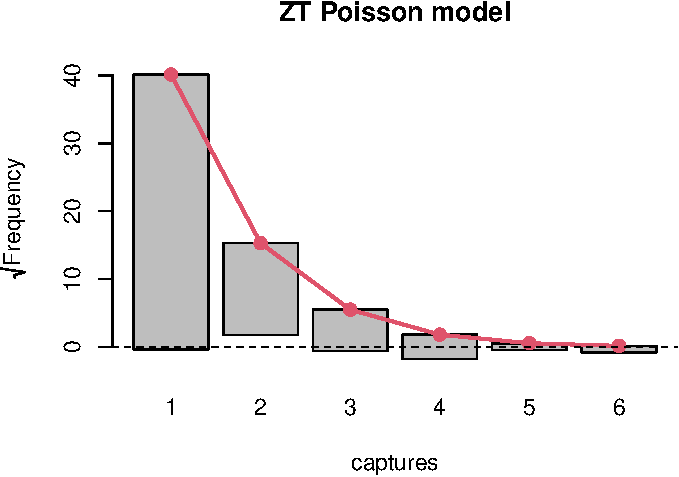
\includegraphics[width=7.5cm]{singleRcapture_files/figure-latex/rootogram-1} 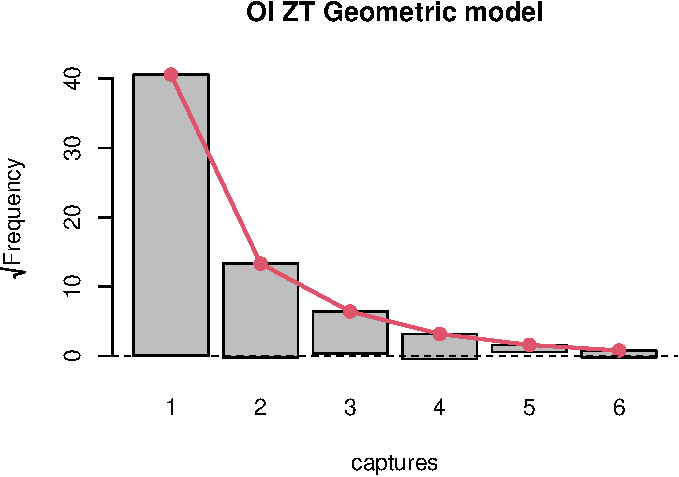
\includegraphics[width=7.5cm]{singleRcapture_files/figure-latex/rootogram-2} \end{center}

\end{CodeChunk}

Plots suggest that the \code{otztgeom} model fits the data better.
Furthermore, important issue in population size estimation is the
diagnostics of the models in order to verify whether influential
observations are present in the data. For this purpose leave-one-out
(LOO) diagnostic implemented in the \code{dfbeta} from the \pkg{stats}
package was adapted and demonstrated below:

\begin{CodeChunk}
\begin{CodeInput}
R> dfb <- dfbeta(basicModel)
R> round(t(apply(dfb, 2, quantile)*100), 4)
\end{CodeInput}
\begin{CodeOutput}
                          0%     25%     50%    75%    100%
(Intercept)          -0.9909 -0.1533  0.0191 0.0521  8.6619
gendermale           -9.0535 -0.0777 -0.0283 0.1017  2.2135
age>40yrs            -2.0010  0.0179  0.0379 0.0691 16.0061
nationAsia           -9.5559 -0.0529  0.0066 0.0120 17.9914
nationNorth Africa   -9.6605 -0.0842 -0.0177 0.0087  3.1260
nationRest of Africa -9.4497 -0.0244  0.0030 0.0083 10.9787
nationSurinam        -9.3138 -0.0065  0.0021 0.0037 99.3383
nationTurkey         -9.6198 -0.0220  0.0079 0.0143 32.0980
\end{CodeOutput}
\end{CodeChunk}

\begin{CodeChunk}
\begin{CodeInput}
R> dfi <- dfbeta(modelInflated)
R> round(t(apply(dfi, 2, quantile)*100), 4)
\end{CodeInput}
\begin{CodeOutput}
                           0%     25%     50%     75%    100%
(Intercept)           -1.4640  0.0050  0.0184  0.0557  9.0600
nationAsia            -6.6331 -0.0346  0.0157  0.0347 12.2406
nationNorth Africa    -7.2770 -0.0768 -0.0170  0.0085  1.9415
nationRest of Africa  -6.6568 -0.0230  0.0081  0.0262  7.1710
nationSurinam         -6.2308 -0.0124  0.0162  0.0421 62.2045
nationTurkey          -6.4795 -0.0273  0.0204  0.0462 21.1338
(Intercept):omega     -6.8668 -0.0193  0.0476  0.0476  9.3389
gendermale:omega      -2.2733 -0.2227  0.1313  0.2482 11.1234
age>40yrs:omega      -30.2130 -0.2247 -0.1312 -0.0663  2.0393
\end{CodeOutput}
\end{CodeChunk}

Furthermore, result of the \code{dfbeta} can be further used in the
function \code{dfpopsize} which allows for quantification of LOO on the
population size.

\begin{CodeChunk}
\begin{CodeInput}
R> dfb_pop <- dfpopsize(basicModel, dfbeta = dfb)
R> dfi_pop <- dfpopsize(modelInflated, dfbeta = dfi)
\end{CodeInput}
\begin{CodeOutput}
Warning in dfpopsize.singleRStaticCountData(modelInflated, dfbeta = dfi):
dfpopsize may (in some cases) not work correctly when bootstrap was chosen as
population variance estimate.
\end{CodeOutput}
\begin{CodeInput}
R> summary(dfb_pop)
\end{CodeInput}
\begin{CodeOutput}
     Min.   1st Qu.    Median      Mean   3rd Qu.      Max. 
-4236.407     2.660     2.660     5.445    17.281   117.445 
\end{CodeOutput}
\begin{CodeInput}
R> summary(dfi_pop)
\end{CodeInput}
\begin{CodeOutput}
     Min.   1st Qu.    Median      Mean   3rd Qu.      Max. 
-456.6443   -3.1121   -0.7243    3.4333    5.1535  103.5949 
\end{CodeOutput}
\end{CodeChunk}

The comparison of deletion effect on population size estimate and
inverse probability weights, which refer to the contribution of a given
observation to the population size estimation, is presented in the
Figure bellow:

\begin{CodeChunk}
\begin{CodeInput}
R> plot(basicModel, plotType = "dfpopContr", dfpop = dfb_pop)
R> plot(modelInflated, plotType = "dfpopContr", dfpop = dfi_pop)
\end{CodeInput}


\begin{center}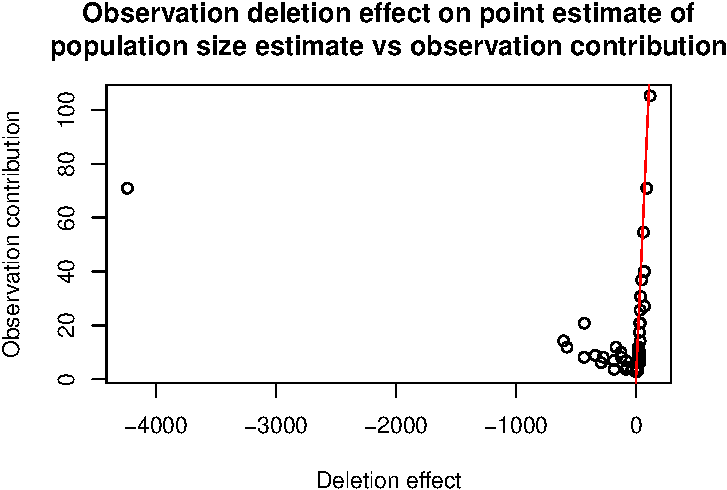
\includegraphics[width=7.5cm]{singleRcapture_files/figure-latex/dfpopsize_plot-1} 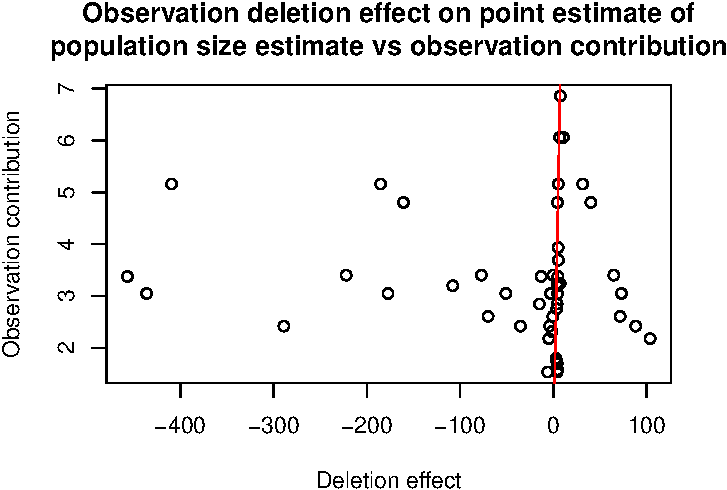
\includegraphics[width=7.5cm]{singleRcapture_files/figure-latex/dfpopsize_plot-2} \end{center}

\end{CodeChunk}

These plot informs on the change of the population size if a given
observation will be removed. For instance if we remove observation 542
from the data then population size will rise by about 4236 for the
\code{ztpoisson} model. While for the \code{oiztgeom} the largest change
is 457 for the 900 observation.

The full list of plot types along with the list of optional arguments
which may be passed from the call to the \code{plot} method down to base
\proglang{R} and \pkg{graphics} functions is listed in the help file of
the \code{plot} method.

\begin{CodeChunk}
\begin{CodeInput}
R> ?plot.singleRStaticCountData
\end{CodeInput}
\end{CodeChunk}

\subsection[The stratifyPopsize function]{The \code{stratifyPopsize} function}

Researchers may be interested on only in the total population size but
also in specific sub-populations (e.g.~males, females, group pages). For
that reason we have created the \code{stratifyPopsize} function which
allows to estimate the size by stratas defined by the coefficients in
the model (the default option). In the output below we present results
based on the \code{ztpoisson} and \code{oiztgeom} models.

\begin{CodeChunk}
\begin{CodeInput}
R> popSizeStratas <- stratifyPopsize(basicModel)
R> cols <- c("name", "Observed", "Estimated", "logNormalLowerBound", 
+           "logNormalUpperBound")
R> popSizeStratas_report <- popSizeStratas[, cols]
R> cols_custom <- c("Name", "Obs", "Estimated", "LowerBound", "UpperBound")
R> names(popSizeStratas_report) <- cols_custom
R> popSizeStratas_report
\end{CodeInput}
\begin{CodeOutput}
                             Name  Obs  Estimated LowerBound UpperBound
1                  gender==female  398  3811.0911  2189.0443   6902.133
2                    gender==male 1482  8879.2594  6090.7762  13354.880
3                     age==<40yrs 1769 10506.8971  7359.4155  15426.455
4                     age==>40yrs  111  2183.4535   872.0130   5754.876
5  nation==American and Australia  173   708.3688   504.6086   1037.331
6                    nation==Asia  284  2742.3147  1755.2548   4391.590
7            nation==North Africa 1023  3055.2033  2697.4900   3489.333
8          nation==Rest of Africa  243  2058.1533  1318.7466   3305.786
9                 nation==Surinam   64  2386.4513   505.2457  12287.983
10                 nation==Turkey   93  1739.8592   638.0497   5068.959
\end{CodeOutput}
\end{CodeChunk}

\begin{CodeChunk}
\begin{CodeInput}
R> popSizeStratas_inflated <- stratifyPopsize(modelInflated)
R> popSizeStratas_inflated_report <- popSizeStratas_inflated[, cols]
R> names(popSizeStratas_inflated_report) <- cols_custom
R> popSizeStratas_inflated_report
\end{CodeInput}
\begin{CodeOutput}
                             Name  Obs Estimated LowerBound UpperBound
1  nation==American and Australia  173  516.2432   370.8463   768.4919
2                    nation==Asia  284 1323.5377   831.1601  2258.9954
3            nation==North Africa 1023 2975.8801  2254.7071  4119.3050
4          nation==Rest of Africa  243 1033.9753   667.6106  1716.4484
5                 nation==Surinam   64  354.2236   193.8891   712.4739
6                  nation==Turkey   93  496.0934   283.1444   947.5309
7                  gender==female  398 1109.7768   778.7197  1728.7066
8                    gender==male 1482 5590.1764  3838.4550  8644.0776
9                     age==<40yrs 1769 6437.8154  4462.3472  9862.2147
10                    age==>40yrs  111  262.1379   170.9490   492.0347
\end{CodeOutput}
\end{CodeChunk}

The function \code{stratifyPopsize}, that is prepared for the objects of
the \code{singleRStaticCountData} class, accepts three optional
parameters \code{stratas, alpha, cov} which correspond to specification
of sub-populations, the significance levels and the covariance matrix
that will be used to compute standard errors. An example of the full
call is presented below.

\begin{CodeChunk}
\begin{CodeInput}
R> library(sandwich)
R> popSizeStratasCustom <- stratifyPopsize(
+   object  = basicModel,
+   stratas = ~ gender + age, 
+   alpha   = rep(c(0.1, 0.05), each=2), 
+   cov     = vcovHC(basicModel, type = "HC4")
+ )
R> 
R> popSizeStratasCustom_report <- popSizeStratasCustom[, c(cols, "confLevel")]
R> names(popSizeStratasCustom_report) <- c(cols_custom, "alpha")
R> popSizeStratasCustom_report
\end{CodeInput}
\begin{CodeOutput}
            Name  Obs Estimated LowerBound UpperBound alpha
1 gender==female  398  3811.091  2275.6416   6602.161  0.10
2   gender==male 1482  8879.259  6261.5125  12930.751  0.10
3    age==<40yrs 1769 10506.897  7297.2081  15580.138  0.05
4    age==>40yrs  111  2183.453   787.0676   6464.009  0.05
\end{CodeOutput}
\end{CodeChunk}

We provide integration with the \pkg{sandwich} \citep{sandwich} package
to correct variance-covariance matrix in the \(\delta\) method. In the
code we have used the \code{vcovHC} method for
\code{singleRStaticCountData} class from the \pkg{sandwich} package,
different significance levels for confidence intervals in each strata
and a formula to specify that we wanted estimates for both males and
females subdivided by \code{nation} and \code{age}. The \code{stratas}
parameter may be specified either as:

\begin{itemize}
\item a formula with empty left hand side which we have seen here (e.g. \code{~ gender * age}),
\item a logical vector with number of entries equal to number of rows in the dataset in which case only one strata will be created (e.g. \code{netherlandsimmigrant$gender == "male"}),
\item a (named) list where each element is a logical vector, names of the list will be used to specify names variable in returned object (e.g. \code{list("Strata 1" = netherlandsimmigrant$gender == "male" 
\& netherlandsimmigrant$nation == "Suriname", 
"Strata 2" = netherlandsimmigrant$gender == "female" 
\& netherlandsimmigrant$nation == "North Africa")}),
\item a vector of names of explanatory variables which will result in every level of explanatory variable having its own sub population for each variable specified (e.g. \code{c("gender", "age")}),
\item or not supplied at all in which case stratas will correspond to levels of each factor in the data without any interactions (string vectors will be converted to factors for the convenience of the user).
\end{itemize}

One may also specify \code{plotType = "strata"} in the \code{plot}
function which results in a plot with point and CI estimates of the
population size.

\begin{CodeChunk}
\begin{CodeInput}
R> par(mar = c(2.5, 8.5, 4.1, 2.5), cex.main = .7, cex.lab = .6)
R> plot(basicModel, plotType = "strata")
R> plot(modelInflated, plotType = "strata")
\end{CodeInput}


\begin{center}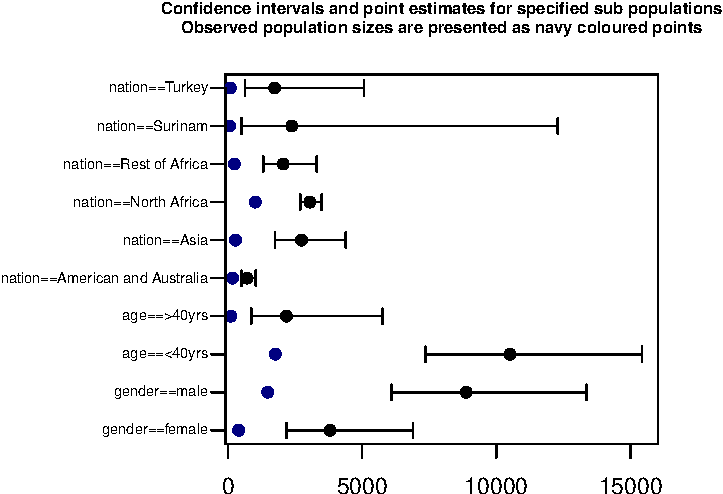
\includegraphics[width=7.5cm]{singleRcapture_files/figure-latex/strata_plot-1} 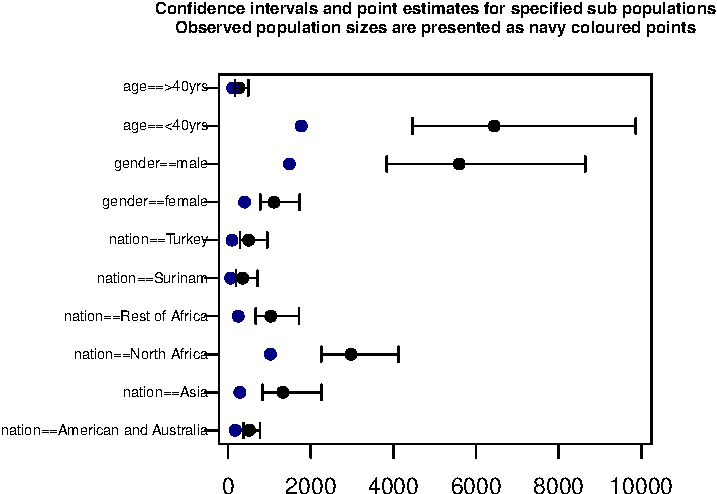
\includegraphics[width=7.5cm]{singleRcapture_files/figure-latex/strata_plot-2} \end{center}

\end{CodeChunk}

For plotting only the \code{logNormal} type of confidence interval is
used since the studentized confidence intervals often result in negative
lower bounds.

\section{Classes and methods}\label{sec-methods}

For the purpose of the package we have created classes
\code{singleRStaticCountData}, \code{singleR} (for now the two former
classes are the same, the distinction is made for future development),
\code{singleRfamily}, \code{popSizeEstResults},
\code{summarysingleRStaticCountData} and \code{summarysingleRmargin}
which allows for extracting relevant information regarding the
population size.

For instance, function \code{popSizeEst} allows to extract information
on the estimated size of the population as given below:

\begin{CodeChunk}
\begin{CodeInput}
R> (popEst <- popSizeEst(basicModel))
\end{CodeInput}
\begin{CodeOutput}
Point estimate: 12690.35
Variance: 7885790
95% confidence intervals:
          lowerBound upperBound
normal      7186.449   18194.25
logNormal   8431.277   19718.31
\end{CodeOutput}
\end{CodeChunk}

and the resulting object \code{popEst} is of the
\code{popSizeEstResults} class contains the following fields:

\begin{itemize}
  \item \code{pointEstimate}, \code{variance} -- numerics containing point estimate and variance of this estimate.
  \item \code{confidenceInterval} -- a \code{data.frame} with confidence intervals.
  \item \code{boot} -- If bootstrap was performed a numeric vector containing the $\hat{N}$ values from the bootstrap, 
  a character vector with value \code{"No bootstrap performed"} otherwise.
  \item \code{control} -- a \code{controlPopVar} object with controls used to obtained the object.
\end{itemize}

The only explicitly defined method for \code{popSizeEstResults},
\code{summarysingleRmargin} and \code{summarysingleRStaticCountData}
classes is the \code{print} method, but the former one also accepts
\proglang{R} primitives like \code{coef}:

\begin{CodeChunk}
\begin{CodeInput}
R> coef(summary(basicModel))
\end{CodeInput}
\begin{CodeOutput}
                       Estimate Std. Error    z value      P(>|z|)
(Intercept)          -1.3410661  0.2148870 -6.2407965 4.353484e-10
gendermale            0.3971793  0.1630155  2.4364504 1.483220e-02
age>40yrs            -0.9746058  0.4082420 -2.3873235 1.697155e-02
nationAsia           -1.0925990  0.3016259 -3.6223642 2.919228e-04
nationNorth Africa    0.1899980  0.1940007  0.9793677 3.273983e-01
nationRest of Africa -0.9106361  0.3008092 -3.0272880 2.467587e-03
nationSurinam        -2.3363949  1.0135639 -2.3051284 2.115938e-02
nationTurkey         -1.6753917  0.6027744 -2.7794674 5.444812e-03
\end{CodeOutput}
\end{CodeChunk}

analogously to \code{glm} from \pkg{stats}. The \code{singleRfamily}
inherits the \code{family} class from \pkg{stats} and has explicitly
defined \code{print} and \code{simulate} methods defined. Example usage
is presented below

\begin{CodeChunk}
\begin{CodeInput}
R> set.seed(1234567890)
R> N <- 10000
R> gender <- rbinom(N, 1, 0.2)
R> eta <- -1 + 0.5*gender
R> counts <- simulate(ztpoisson(), eta = cbind(eta), seed = 1)
R> summary(data.frame(gender, eta, counts))
\end{CodeInput}
\begin{CodeOutput}
     gender            eta              counts      
 Min.   :0.0000   Min.   :-1.0000   Min.   :0.0000  
 1st Qu.:0.0000   1st Qu.:-1.0000   1st Qu.:0.0000  
 Median :0.0000   Median :-1.0000   Median :0.0000  
 Mean   :0.2036   Mean   :-0.8982   Mean   :0.4196  
 3rd Qu.:0.0000   3rd Qu.:-1.0000   3rd Qu.:1.0000  
 Max.   :1.0000   Max.   :-0.5000   Max.   :5.0000  
\end{CodeOutput}
\end{CodeChunk}

The full list of explicitly defined methods for
\code{singleRStaticCountData} methods is

\begin{table}[ht!]
\centering
\small
\begin{tabular}{p{4cm}p{11cm}}
\hline 
Function & Description \\
\hline
\code{fitted} & Which work almost exactly like \code{glm} counterparts but return more information, namely on fitted values for the truncated and non-truncated probability distribution. \\
\code{logLik} & which compared to \code{glm} method has the possibility of returning not just the value of the fitted log-likelihood but also the entire function (argument \code{type = "function"}) along with two first derivatives (argument \code{deriv = 0:2}) \\
\code{model.matrix} & which has the possibility of returning the $X_{\text{vlm}}$ matrix defined in \ref{X_vlm-definition}\\
\code{simulate} & which calls \code{simulate} method for the chosen model and fitted $\boldsymbol{\eta}$ \\
\code{predict} &  which has the possibility of returning either of fitted ditribution parameters for each unit (\code{type = "response"}), just linear predictors (\code{type = "link"}), means of the fitted distributnios of $Y$ and $Y|Y>0$ (\code{type = "mean"}) and the inverse probability weights (\code{type = "contr"}). There us also the \code{se.fit} argument which can be set to \code{TRUE} to obtain standard errors for each of those by using the $\delta$ method. Also it is possible to use a custom covariance matrix for standard error computation (argument \code{cov}). \\
\code{redoPopEstimation} & A function that applies all post-hoc procedures that were taken (such as heteroscedastic consistent covariance matrix estimation via \pkg{countreg}) to population size estimation and standard error estimation. \\
\code{residuals} & for obtaining residuals of several types, we refer interested readers to the manual \code{?singleRcapture:::residuals.singleRStaticCountData}. \\
\code{stratifyPopsize, summary} & which were already discussed. Compared to \code{glm} class summary has the possibility of adding confidence interval to the coefficient matrix (argument \code{confint = TRUE}) and using custom covariance matrix (argument \code{cov = someMatrix}) \\
\code{plot} & which was already discussed \\
\code{popSizeEst} & an extractor showcased above. \\
\code{cooks.distance} & which works only for single predictor models \\
\code{dfbeta, dfpopsize} & Multithreading in \code{dfbeta} is available and \code{dfpopsize} calls \code{dfbeta} if no \code{dfbeta} object was provided at call. \\
\code{bread, estfun, vcovHC} & for (almost) full \pkg{sandwich} compatibility. \\
\code{AIC, BIC, extractAIC, family, confint, df.residual, model.frame, hatvalues, nobs, print}  & Which work exactly like \code{glm} counterparts.\\
\hline 
\end{tabular}
\caption{\code{S3Methods} implemented in the \pkg{singleRcapture}}
\end{table}

\section[Integration with the]{Integration with the \pkg{VGAM, countreg}
packages}\label{sec-vgam}

As noted at the beginning we provide an integration with the \pkg{VGAM}
and \pkg{countreg} packages via the \pkg{singleRcaptureExtra} package
available through Github at
\url{https://github.com/ncn-foreigners/singleRcaptureExtra}.

\begin{CodeChunk}
\begin{CodeInput}
R> install.packages("pak")
R> pak::pak("ncn-foreigners/singleRcaptureExtra")
\end{CodeInput}
\end{CodeChunk}

The \pkg{singleRcaptureExtra} allows for converting objects created by
\code{vglm, vgam, countreg} functions from packages \pkg{VGAM, countreg}
to a \code{singleRStaticCountData} via the respective
\code{estimatePopsize} methods for their classes. The help files for all
the methods and all the control functions are accessed by

\begin{CodeChunk}
\begin{CodeInput}
R> ?estimatePopsize.vgam
R> ?controlEstPopVgam
\end{CodeInput}
\end{CodeChunk}

Using the fitted \code{zerotrunc, vglm, vgam} class objects in
population size estimation such as the one additive models with smooth
terms for dataset from \cite{chao-generalization}. Note that we use a
different dataset than the one presented in the case study as our goal
is to show usage of additive models and how it handled in the
\pkg{singleRcapture} package.

\begin{CodeChunk}
\begin{CodeInput}
R> library(VGAM)
R> library(singleRcaptureExtra)
R> modelVgam <- vgam(
+   TOTAL_SUB ~ (s(log_size, df  = 3) + s(log_distance, df  = 2)) / C_TYPE,
+   data = farmsubmission,
+   # Using different link since
+   # VGAM uses parametrisation with 1/alpha
+   family = posnegbinomial(
+     lsize = negloglink
+   )
+ )
\end{CodeInput}
\end{CodeChunk}

Estimation of the population size can be accomplished with the following
syntax simple syntax.

\begin{CodeChunk}
\begin{CodeInput}
R> modelVgamPop <- estimatePopsize(modelVgam)
\end{CodeInput}
\end{CodeChunk}

The resulting object is of class \code{singleRforeign} to underline that
the parameters were estimated outside the \pkg{singleRcapture}.
Resulting object consist of the following elements

\begin{CodeChunk}
\begin{CodeInput}
R> str(modelVgamPop,1)
\end{CodeInput}
\begin{CodeOutput}
List of 5
 $ foreignObject :Formal class 'vgam' [package "VGAM"] with 43 slots
 $ call          : language estimatePopsize.vgam(formula = modelVgam)
 $ sizeObserved  : int 12036
 $ populationSize:List of 5
  ..- attr(*, "class")= chr "popSizeEstResults"
 $ derivFunc     :function (eta)  
 - attr(*, "class")= chr [1:4] "singleRadditive" "singleRforeign" "singleRStaticCountData" "singleR"
\end{CodeOutput}
\end{CodeChunk}

Compare with a similar linear model from base \pkg{singleRcapture}:
\small

\begin{CodeChunk}
\begin{CodeInput}
R> modelBase <- estimatePopsize(
+   TOTAL_SUB ~ (log_size + log_distance) * C_TYPE,
+   data = farmsubmission,
+   model = ztnegbin()
+ )
R> summary(modelBase)
\end{CodeInput}
\begin{CodeOutput}

Call:
estimatePopsize.default(formula = TOTAL_SUB ~ (log_size + log_distance) * 
    C_TYPE, data = farmsubmission, model = ztnegbin())

Pearson Residuals:
     Min.   1st Qu.    Median      Mean   3rd Qu.      Max. 
-0.729357 -0.317558 -0.152482  0.000609  0.148985  6.604269 

Coefficients:
-----------------------
For linear predictors associated with: lambda 
                         Estimate Std. Error z value  P(>|z|)    
(Intercept)              -1.77609    0.45894  -3.870 0.000109 ***
log_size                  0.49391    0.02521  19.594  < 2e-16 ***
log_distance             -0.14106    0.04098  -3.442 0.000578 ***
C_TYPEDairy              -1.68591    0.55327  -3.047 0.002310 ** 
log_size:C_TYPEDairy      0.26504    0.03495   7.583 3.37e-14 ***
log_distance:C_TYPEDairy  0.08568    0.04874   1.758 0.078762 .  
-----------------------
For linear predictors associated with: alpha 
            Estimate Std. Error z value  P(>|z|)    
(Intercept)  0.57673    0.07267   7.936 2.09e-15 ***
---
Signif. codes:  0 '***' 0.001 '**' 0.01 '*' 0.05 '.' 0.1 ' ' 1

AIC: 34481.99
BIC: 34533.76
Residual deviance: 17611.16

Log-likelihood: -17233.99 on 24065 Degrees of freedom 
Number of iterations: 9
-----------------------
Population size estimation results: 
Point estimate 38877
Observed proportion: 31% (N obs = 12036)
Std. Error 1749.448
95% CI for the population size:
          lowerBound upperBound
normal      35448.14   42305.85
logNormal   35661.32   42530.37
95% CI for the share of observed population:
          lowerBound upperBound
normal      28.44996   33.95382
logNormal   28.29978   33.75085
\end{CodeOutput}
\begin{CodeInput}
R> summary(modelVgamPop)
\end{CodeInput}
\begin{CodeOutput}

Call:
estimatePopsize.vgam(formula = modelVgam)

-----------------------
Population size estimation results: 
Point estimate 37760.01
Observed proportion: 31.9% (N obs = 12036)
Std. Error 1630.429
95% CI for the population size:
          lowerBound upperBound
normal      34564.42   40955.59
logNormal   34757.77   41158.93
95% CI for the share of observed population:
          lowerBound upperBound
normal      29.38793   34.82193
logNormal   29.24274   34.62823

-------------------------------
-- Summary of foreign object --
-------------------------------

Call:
vgam(formula = TOTAL_SUB ~ (s(log_size, df = 3) + s(log_distance, 
    df = 2))/C_TYPE, family = posnegbinomial(lsize = negloglink), 
    data = farmsubmission)

Names of additive predictors: loglink(munb), negloglink(size)

Dispersion Parameter for posnegbinomial family:   1

Log-likelihood: -17214.62 on 24063.17 degrees of freedom

Number of Fisher scoring iterations:  11 

DF for Terms and Approximate Chi-squares for Nonparametric Effects

                                                   Df Npar Df Npar Chisq
(Intercept):1                                       1                   
(Intercept):2                                       1                   
s(log_size, df = 3)                                 1     1.8     51.949
s(log_distance, df = 2)                             1     1.0      3.503
s(log_size, df = 3):s(log_distance, df = 2):C_TYPE  2                   
                                                     P(Chi)
(Intercept):1                                              
(Intercept):2                                              
s(log_size, df = 3)                                0.000000
s(log_distance, df = 2)                            0.063835
s(log_size, df = 3):s(log_distance, df = 2):C_TYPE         
\end{CodeOutput}
\end{CodeChunk}

\normalsize

\section{Concluding remarks}\label{concluding-remarks}

In this paper we have introduced two packages for single source
capture-recapture models, namely \pkg{singleRcapture} and
\pkg{singleRcaptureExtra}. The packages implement state of the art
methods for estimating population size based on a single data set with
multiple counts. The package allows for different methods to account for
heterogeneity in capture probabilities, modelled using covariates, as
well as behavioural change, modelled using one-inflation. We have build
the package in a such way that it is easy to implement new models using
\code{family} objects which is demonstrated in the Appendix
\ref{sec-family}.

In future work we plan to consider Bayesian estimation using
\proglang{Stan} (e.g.~via the \pkg{brms} package;
\cite{carpenter2017stan, brms}) and for one-inflation models we may use
the recent approach proposed by \cite{tuoto2022bayesian} and implement
our own families using the \pkg{brms} package.

\section{Acknowledgements}\label{Acknowledgements}

The authors' work has been financed by the National Science Centre in
Poland, OPUS 20, grant no. 2020/39/B/HS4/00941.

The authors would like to thank Peter van der Heijden, Maarten Cruyff,
Dankmar Böhning and Layna Dennett for useful comments that led to the
improved of the functionality of the package. In addition we would like
to thank Tymon Świtalski for valuable comments that improved the paper.

\appendix

\section{Detailed information}\label{sec-details}

\subsection[The estimatePopsizeFit function]{The
\code{estimatePopsizeFit} function}\label{sec-estimatePopsizeFit}

In this section we provide step-by-step description how to prepare data
to use the \code{estimatePopsizeFit} function that may be useful for
instance for estimation of variance.

\begin{enumerate}
\def\labelenumi{\arabic{enumi}.}
\tightlist
\item
  Create data matrix \(\boldsymbol{X}_{vlm}\)
\end{enumerate}

\begin{CodeChunk}
\begin{CodeInput}
R> X <- matrix(data = 0, nrow = 2 * NROW(farmsubmission), ncol = 7)
\end{CodeInput}
\end{CodeChunk}

\begin{enumerate}
\def\labelenumi{\arabic{enumi}.}
\setcounter{enumi}{1}
\tightlist
\item
  Fill the first \(n\) rows with \code{model.matrix} according to the
  specified formula and specify the attribute \code{attr(X, "hwm")} that
  informs the function which elements of the design matrix correspond to
  which linear predictor (covariates for counts and covariates for
  one-inflation)
\end{enumerate}

\begin{CodeChunk}
\begin{CodeInput}
R> X[1:NROW(farmsubmission), 1:4] <- model.matrix(
+   ~ 1 + log_size + log_distance + C_TYPE, 
+   farmsubmission
+ )
R> X[-(1:NROW(farmsubmission)), 5:7] <- model.matrix(
+   ~ 1 + log_distance + C_TYPE, 
+   farmsubmission
+ )
R> 
R> attr(X, "hwm") <- c(4, 3)
\end{CodeInput}
\end{CodeChunk}

\begin{enumerate}
\def\labelenumi{\arabic{enumi}.}
\setcounter{enumi}{2}
\tightlist
\item
  Obtain starting \(\boldsymbol{\beta}\) parameters using \code{glm.fit}
  function.
\end{enumerate}

\begin{CodeChunk}
\begin{CodeInput}
R> start <- glm.fit(# get starting points
+   y = farmsubmission$TOTAL_SUB, 
+   x = X[1:NROW(farmsubmission), 1:4], 
+   family = poisson()
+ )$coefficients
R> 
R> start
\end{CodeInput}
\begin{CodeOutput}
[1] -0.82583943  0.33254499 -0.03277732  0.32746933
\end{CodeOutput}
\end{CodeChunk}

\begin{enumerate}
\def\labelenumi{\arabic{enumi}.}
\setcounter{enumi}{3}
\tightlist
\item
  Use \code{estimatePopsizeFit} function to fit the model assuming
  zero-truncated one-inflated geometric distribution as specified in the
  \code{family} argument.
\end{enumerate}

\begin{CodeChunk}
\begin{CodeInput}
R> res <- estimatePopsizeFit(
+   y            = farmsubmission$TOTAL_SUB, 
+   X            = X, 
+   method       = "IRLS", 
+   priorWeights = 1, 
+   family       = ztoigeom(), 
+   control      = controlMethod(silent = TRUE), 
+   coefStart    = c(start, 0, 0, 0),
+   etaStart     = matrix(X %*% c(start, 0, 0, 0), ncol = 2),
+   offset       = cbind(rep(0, NROW(farmsubmission)), 
+                        rep(0, NROW(farmsubmission)))
+ )
\end{CodeInput}
\end{CodeChunk}

\begin{enumerate}
\def\labelenumi{\arabic{enumi}.}
\setcounter{enumi}{4}
\tightlist
\item
  Compare our results with those from \code{stats::optim} function.
\end{enumerate}

\begin{CodeChunk}
\begin{CodeInput}
R> ll <- ztoigeom()$makeMinusLogLike(y = farmsubmission$TOTAL_SUB, X = X)
\end{CodeInput}
\end{CodeChunk}

\begin{CodeChunk}
\begin{CodeInput}
R> res2 <- estimatePopsizeFit(
+   y = farmsubmission$TOTAL_SUB, 
+   X = X, 
+   method = "optim", 
+   priorWeights = 1, 
+   family = ztoigeom(), 
+   coefStart = c(start, 0, 0, 0),
+   control = controlMethod(silent = TRUE),
+   offset = cbind(rep(0, NROW(farmsubmission)), rep(0, NROW(farmsubmission)))
+ )
\end{CodeInput}
\end{CodeChunk}

\begin{CodeChunk}
\begin{CodeInput}
R> data.frame(singleRcapture = round(c(res$beta, -ll(res$beta), res$iter), 4),
+            optim = round(c(res2$beta, -ll(res2$beta), res2$iter[1]), 4))
\end{CodeInput}
\begin{CodeOutput}
  singleRcapture       optim
1        -2.7845     -2.6408
2         0.6170      0.6258
3        -0.0646     -0.0829
4         0.5346      0.5325
5        -3.1745     -0.1244
6         0.1281     -0.1630
7        -1.0865     -1.1055
8    -17278.7613 -17280.3414
9        15.0000   1002.0000
\end{CodeOutput}
\end{CodeChunk}

\clearpage

\subsection{Structure of a family function}\label{sec-family}

In this section we provide details on the \code{family} object for the
\pkg{singleRcapture} package. This object contains additional parameters
in comparison to the standard \code{family} object from the \code{stats}
package.

\begin{table}[ht!]
\centering
\small
\begin{tabular}{p{4cm}p{11cm}}
\hline 
Function & Description \\
\hline
\code{makeMinusLogLike} & 
A factory function for creating the:
  \begin{equation*}
    \ell(\boldsymbol{\beta}), 
    \frac{\partial\ell}{\partial\boldsymbol{\beta}},
    \frac{\partial^{2}\ell}{\partial\boldsymbol{\beta}^\top\partial\boldsymbol{\beta}}
  \end{equation*}
  functions from $\boldsymbol{y}$ vector and $\boldsymbol{X}_{vlm}$ the argument \code{deriv} with possible 
  values in \code{c(0, 1, 2)} provides which derivative to return with the default \code{0} being just the minus log-likelihood \\
\code{links} & List with link functions \\
\code{mu.eta, variance} & Functions of linear predictors that return expected value and variance. There is a `type` argument with 2 possible values \code{"trunc"} and \code{"nontrunc"} that specifies whether to return $\mathbb{E}[Y|Y>0], \text{var}[Y|Y>0]$ or $\mathbb{E}[Y], \text{var}[Y]$ respectively, also the \code{deriv} argument with values in \code{c(0, 1, 2)} is used for indicating the derivative with respect to the linear predictors with is used for providing standard error in \code{predict} method \\
\code{family} & Character that specifies name of the model \\
\code{valideta, validmu} & For now only returns true. In near future will be used to check whether applied linear predictors are valid (i.e. are transformed into some elements of parameter space the subjected to inverse link function) \\
\code{funcZ, Wfun} & Functions that create pseudo residuals and working weights used in IRLS algorithm \\
\code{devResids}  & Function that given the linear predictors prior weights vector and response vector returns deviance residuals \\
\code{pointEst, popVar} & Functions that given prior weights linear predictors and in the later case also estimation of  $\text{cov}(\hat{\boldsymbol{\beta}})$ and $\boldsymbol{X_{vlm}}$ matrix return point estimate for population size and analytic estimation of its variance.There is a additional boolean parameter \code{contr} in the former function that if set to true returns contribution of each unit \\
\code{etaNames} & Names of linear predictors \\
\code{densityFunction} & A function that given linear predictors returns value of PMF at values \code{x}. Additional argument \code{type} specifies whether to return $\mathbb{P}[Y|Y>0]$ or $\mathbb{P}[Y]$ \\
\code{simulate} & A function that generates values of dependent  vector given linear predictors \\
\code{getStart} & Expression for generating starting points \\
\hline
\end{tabular}
\end{table}

\clearpage

\section[Implementing custom singleRcapture family function]{Implementing
custom \pkg{singleRcapture} family
function}\label{implementing-custom-family-function}

Suppose we want to implement a very specific zero truncated family
function in the \pkg{singleRcapture} which corresponds to the following
``untruncated'' distribution: \begin{equation}
  \mathbb{P}[Y=y|\lambda, \pi] = \begin{cases}
    1 - \frac{1}{2}\lambda - \frac{1}{2}\pi & \text{when: } y=0\\
    \frac{1}{2}\pi & \text{when: } y=1\\
    \frac{1}{2}\lambda & \text{when: } y=2,
  \end{cases}
\end{equation} with \(\lambda, \pi\in\left(0, 1\right)\) being dependent
on covariates.

The following would be one way of implementing it, with
\code{lambda, pi} in the code meaning
\(\frac{1}{2}\lambda,\frac{1}{2}\pi\) in the equation above.

\small

\begin{CodeChunk}
\begin{CodeInput}
R> myFamilyFunction <- function(lambdaLink = c("logit", "cloglog", "probit"),
+                              piLink     = c("logit", "cloglog", "probit"),
+                              ...) {
+   if (missing(lambdaLink)) lambdaLink <- "logit"
+   if (missing(piLink))         piLink <- "logit"
+   
+   links <- list()
+   attr(links, "linkNames") <- c(lambdaLink, piLink)
+   
+   lambdaLink <- switch(lambdaLink,
+     "logit"   = singleRcapture:::singleRinternallogitLink,
+     "cloglog" = singleRcapture:::singleRinternalcloglogLink,
+     "probit"  = singleRcapture:::singleRinternalprobitLink
+   )
+   
+   piLink <- switch(piLink,
+     "logit"   = singleRcapture:::singleRinternallogitLink,
+     "cloglog" = singleRcapture:::singleRinternalcloglogLink,
+     "probit"  = singleRcapture:::singleRinternalprobitLink
+   )
+   
+   links[1:2] <- c(lambdaLink, piLink)
+ 
+   mu.eta <- function(eta, type = "trunc", deriv = FALSE, ...) {
+     pi     <-     piLink(eta[, 2], inverse = TRUE) / 2
+     lambda <- lambdaLink(eta[, 1], inverse = TRUE) / 2
+     
+     if (!deriv) {
+       switch (type,
+         "nontrunc" = pi + 2 * lambda,
+         "trunc" = 1 + lambda / (pi + lambda)
+       )
+     } else {
+       # Only necessary if one wishes to use standard errors in predict method
+       switch (type,
+         "nontrunc" = {
+           matrix(c(2, 1) * c(
+             lambdaLink(eta[, 1], inverse = TRUE, deriv = 1) / 2,
+                 piLink(eta[, 2], inverse = TRUE, deriv = 1) / 2
+           ), ncol = 2)
+         },
+         "trunc" = {
+           matrix(c(
+             pi / (pi + lambda) ^ 2,
+             -lambda / (pi + lambda) ^ 2
+           ) * c(
+             lambdaLink(eta[, 1], inverse = TRUE, deriv = 1) / 2,
+                 piLink(eta[, 2], inverse = TRUE, deriv = 1) / 2
+           ), ncol = 2)
+         }
+       )
+     }
+   }
+   
+   variance <- function(eta, type = "nontrunc", ...) {
+     pi     <-     piLink(eta[, 2], inverse = TRUE) / 2
+     lambda <- lambdaLink(eta[, 1], inverse = TRUE) / 2
+     
+     switch (type,
+     "nontrunc" = pi * (1 - pi) + 4 * lambda * (1 - lambda - pi),
+     "trunc" = lambda * (1 - lambda) / (pi + lambda)
+     )
+   }
+   
+   Wfun <- function(prior, y, eta, ...) {
+     pi     <-     piLink(eta[, 2], inverse = TRUE) / 2
+     lambda <- lambdaLink(eta[, 1], inverse = TRUE) / 2
+     
+     G01 <- ((lambda + pi) ^ (-2)) * piLink(eta[, 2], inverse = TRUE, deriv = 1) *
+       lambdaLink(eta[, 1], inverse = TRUE, deriv = 1) * prior / 4
+     
+     G00 <- ((lambda + pi) ^ (-2)) - (pi ^ (-2)) - lambda / ((lambda + pi) * (pi ^ 2))
+     G00 <- G00 * prior * (piLink(eta[, 2], inverse = TRUE, deriv = 1) ^ 2) / 4
+     
+     G11 <- ((lambda + pi) ^ (-2)) - (((lambda + pi) * lambda) ^ -1)
+     G11 <- G11 * prior * (lambdaLink(eta[, 1], inverse = TRUE, deriv = 1) ^ 2) / 4
+     
+     matrix(
+       -c(G11, # lambda
+          G01, # mixed
+          G01, # mixed
+          G00  # pi
+       ),
+       dimnames = list(rownames(eta), c("lambda", "mixed", "mixed", "pi")),
+       ncol = 4
+     )
+   }
+   
+   funcZ <- function(eta, weight, y, prior, ...) {
+     pi     <-     piLink(eta[, 2], inverse = TRUE) / 2
+     lambda <- lambdaLink(eta[, 1], inverse = TRUE) / 2
+     
+     weight <- weight / prior
+     
+     G0 <- (2 - y) / pi     - ((lambda + pi) ^ -1)
+     G1 <- (y - 1) / lambda - ((lambda + pi) ^ -1)
+     
+     G1 <- G1 * lambdaLink(eta[, 1], inverse = TRUE, deriv = 1) / 2
+     G0 <- G0 *     piLink(eta[, 2], inverse = TRUE, deriv = 1) / 2
+     
+     uMatrix <- matrix(c(G1, G0), ncol = 2)
+     
+     weight <- lapply(X = 1:nrow(weight), FUN = function (x) {
+       matrix(as.numeric(weight[x, ]), ncol = 2)
+     })
+     
+     pseudoResid <- sapply(X = 1:length(weight), FUN = function (x) {
+       #xx <- chol2inv(chol(weight[[x]])) # less computationally demanding
+       xx <- solve(weight[[x]]) # more stable
+       xx %*% uMatrix[x, ]
+     })
+     pseudoResid <- t(pseudoResid)
+     dimnames(pseudoResid) <- dimnames(eta)
+     pseudoResid
+   }
+   
+   minusLogLike <- function(y, X, offset,
+                            weight    = 1, 
+                            NbyK      = FALSE, 
+                            vectorDer = FALSE, 
+                            deriv     = 0, 
+                            ...) {
+     y <- as.numeric(y)
+     if (is.null(weight)) {
+       weight <- 1
+     }
+     if (missing(offset)) {
+       offset <- cbind(rep(0, NROW(X) / 2), rep(0, NROW(X) / 2))
+     }
+     
+     if (!(deriv %in% c(0, 1, 2))) 
+       stop("Only score function and derivatives up to 2 are supported.")
+     deriv <- deriv + 1 
+     
+     switch (deriv,
+       function(beta) {
+         eta <- matrix(as.matrix(X) %*% beta, ncol = 2) + offset
+         pi     <-     piLink(eta[, 2], inverse = TRUE) / 2
+         lambda <- lambdaLink(eta[, 1], inverse = TRUE) / 2
+         -sum(weight * ((2 - y) * log(pi) + (y - 1) * log(lambda) - log(pi + lambda)))
+       },
+       function(beta) {
+         eta <- matrix(as.matrix(X) %*% beta, ncol = 2) + offset
+         pi     <-     piLink(eta[, 2], inverse = TRUE) / 2
+         lambda <- lambdaLink(eta[, 1], inverse = TRUE) / 2
+         
+         G0 <- (2 - y) / pi     - ((lambda + pi) ^ -1)
+         G1 <- (y - 1) / lambda - ((lambda + pi) ^ -1)
+         
+         G1 <- G1 * weight * lambdaLink(eta[, 1], inverse = TRUE, deriv = 1) / 2
+         G0 <- G0 * weight *     piLink(eta[, 2], inverse = TRUE, deriv = 1) / 2
+         
+         if (NbyK) {
+           XX <- 1:(attr(X, "hwm")[1])
+           return(cbind(as.data.frame(X[1:nrow(eta), XX]) * G1,
+                        as.data.frame(X[-(1:nrow(eta)), -XX]) * G0))
+         }
+         if (vectorDer) {
+           return(cbind(G1, G0))
+         }
+         
+         as.numeric(c(G1, G0) %*% X)
+       },
+       function (beta) {
+         lambdaPredNumber <- attr(X, "hwm")[1]
+         eta <- matrix(as.matrix(X) %*% beta, ncol = 2) + offset
+         pi     <-     piLink(eta[, 2], inverse = TRUE) / 2
+         lambda <- lambdaLink(eta[, 1], inverse = TRUE) / 2
+ 
+         res <- matrix(nrow = length(beta), ncol = length(beta), 
+                       dimnames = list(names(beta), names(beta)))
+         
+         # pi^2 derivative
+         dpi <- (2 - y) / pi - (lambda + pi) ^ -1
+         G00 <- ((lambda + pi) ^ (-2)) - (2 - y) / (pi ^ 2)
+         
+         G00 <- t(as.data.frame(X[-(1:(nrow(X) / 2)), -(1:lambdaPredNumber)] * 
+         (G00 * ((piLink(eta[, 2], inverse = TRUE, deriv = 1) / 2) ^ 2) + 
+         dpi * piLink(eta[, 2], inverse = TRUE, deriv = 2) / 2) * weight)) %*% 
+         as.matrix(X[-(1:(nrow(X) / 2)), -(1:lambdaPredNumber)])
+         # mixed derivative
+         G01 <- (lambda + pi) ^ (-2)
+         
+         G01 <- t(as.data.frame(X[1:(nrow(X) / 2), 1:lambdaPredNumber]) * 
+         G01 * (lambdaLink(eta[, 1], inverse = TRUE, deriv = 1) / 2) * 
+         (piLink(eta[, 2], inverse = TRUE, deriv = 1) / 2) * weight) %*% 
+         as.matrix(X[-(1:(nrow(X) / 2)), -(1:lambdaPredNumber)])
+         # lambda^2 derivative
+         G11 <- ((lambda + pi) ^ (-2)) - (y - 1) / (lambda ^ 2)
+         dlambda <- (y - 1) / lambda - ((lambda + pi) ^ -1)
+         
+         G11 <- t(as.data.frame(X[1:(nrow(X) / 2), 1:lambdaPredNumber] * 
+         (G11 * ((lambdaLink(eta[, 1], inverse = TRUE, deriv = 1) / 2) ^ 2) + 
+         dlambda * lambdaLink(eta[, 1], inverse = TRUE, deriv = 2) / 2) * weight)) %*% 
+         X[1:(nrow(X) / 2), 1:lambdaPredNumber]
+         
+         res[-(1:lambdaPredNumber), -(1:lambdaPredNumber)] <- G00
+         res[1:lambdaPredNumber, 1:lambdaPredNumber] <- G11
+         res[1:lambdaPredNumber, -(1:lambdaPredNumber)] <- t(G01)
+         res[-(1:lambdaPredNumber), 1:lambdaPredNumber] <- G01
+         
+         res
+       }
+     )
+   }
+   
+   validmu <- function(mu) {
+     (sum(!is.finite(mu)) == 0) && all(0 < mu) && all(2 > mu)
+   }
+   
+   # this is optional
+   devResids <- function(y, eta, wt, ...) {
+     0
+   }
+   
+   pointEst <- function (pw, eta, contr = FALSE, ...) {
+     pi     <-     piLink(eta[, 2], inverse = TRUE) / 2
+     lambda <- lambdaLink(eta[, 1], inverse = TRUE) / 2
+     N <- pw / (lambda + pi)
+     if(!contr) {
+       N <- sum(N)
+     }
+     N
+   }
+   
+   popVar <- function (pw, eta, cov, Xvlm, ...) {
+     pi     <-     piLink(eta[, 2], inverse = TRUE) / 2
+     lambda <- lambdaLink(eta[, 1], inverse = TRUE) / 2
+     
+     bigTheta1 <- -pw / (pi + lambda) ^ 2 # w.r to pi
+     bigTheta1 <- bigTheta1 * piLink(eta[, 2], inverse = TRUE, deriv = 1) / 2
+     bigTheta2 <- -pw / (pi + lambda) ^ 2 # w.r to lambda
+     bigTheta2 <- bigTheta2 * lambdaLink(eta[, 1], inverse = TRUE, deriv = 1) / 2 # w.r to lambda
+     
+     bigTheta <- t(c(bigTheta2, bigTheta1) %*% Xvlm)
+     
+     f1 <- t(bigTheta) %*% as.matrix(cov) %*% bigTheta
+     
+     f2 <- sum(pw * (1 - pi - lambda) / ((pi + lambda) ^ 2))
+     
+     f1 + f2
+   }
+   
+   dFun <- function (x, eta, type = c("trunc", "nontrunc")) {
+     if (missing(type)) type <- "trunc"
+     pi     <-     piLink(eta[, 2], inverse = TRUE) / 2
+     lambda <- lambdaLink(eta[, 1], inverse = TRUE) / 2
+     
+     switch (type,
+       "trunc" = {
+         (pi * as.numeric(x == 1) + lambda * as.numeric(x == 2)) / (pi + lambda)
+       },
+       "nontrunc" = {
+         (1 - pi - lambda) * as.numeric(x == 0) +
+         pi * as.numeric(x == 1) + lambda * as.numeric(x == 2)
+       }
+     )
+   }
+   
+   simulate <- function(n, eta, lower = 0, upper = Inf) {
+     pi     <-     piLink(eta[, 2], inverse = TRUE) / 2
+     lambda <- lambdaLink(eta[, 1], inverse = TRUE) / 2
+     CDF <- function(x) {
+       ifelse(x == Inf, 1, 
+       ifelse(x < 0, 0, 
+       ifelse(x < 1, 1 - pi - lambda,
+       ifelse(x < 2, 1 - lambda, 1))))
+     }
+     lb <- CDF(lower)
+     ub <- CDF(upper)
+     p_u <- stats::runif(n, lb, ub)
+     sims <- rep(0, n)
+     cond <- CDF(sims) <= p_u
+     while (any(cond)) {
+       sims[cond] <- sims[cond] + 1
+       cond <- CDF(sims) <= p_u
+     }
+     sims
+   }
+   
+   getStart <- expression(
+     if (method == "IRLS") {
+       etaStart <- cbind(
+         family$links[[1]](mean(observed == 2) * (1 + 0 * (observed == 2))), # lambda
+         family$links[[2]](mean(observed == 1) * (1 + 0 * (observed == 1)))  # pi
+       ) + offset
+     } else if (method == "optim") {
+       init <- c(
+         family$links[[1]](weighted.mean(observed == 2, priorWeights) * 1 + .0001),
+         family$links[[2]](weighted.mean(observed == 1, priorWeights) * 1 + .0001)
+       )
+       if (attr(terms, "intercept")) {
+         coefStart <- c(init[1], rep(0, attr(Xvlm, "hwm")[1] - 1))
+       } else {
+         coefStart <- rep(init[1] / attr(Xvlm, "hwm")[1], attr(Xvlm, "hwm")[1])
+       }
+       if ("(Intercept):pi" %in% colnames(Xvlm)) {
+         coefStart <- c(coefStart, init[2], rep(0, attr(Xvlm, "hwm")[2] - 1))
+       } else {
+         coefStart <- c(coefStart, rep(init[2] / attr(Xvlm, "hwm")[2], attr(Xvlm, "hwm")[2]))
+       }
+     }
+   )
+   
+   structure(
+     list(
+       makeMinusLogLike = minusLogLike,
+       densityFunction  = dFun,
+       links     = links,
+       mu.eta    = mu.eta,
+       valideta  = function (eta) {TRUE},
+       variance  = variance,
+       Wfun      = Wfun,
+       funcZ     = funcZ,
+       devResids = devResids,
+       validmu   = validmu,
+       pointEst  = pointEst,
+       popVar    = popVar,
+       family    = "myFamilyFunction",
+       etaNames  = c("lambda", "pi"),
+       simulate  = simulate,
+       getStart  = getStart,
+       extraInfo = c(
+         mean       = "pi / 2 + lambda",
+         variance   = paste0("(pi / 2) * (1 - pi / 2) + 2 * lambda * (1 - lambda / 2 - pi / 2)"),
+         popSizeEst = "(1 - (pi + lambda) / 2) ^ -1",
+         meanTr     = "1 + lambda / (pi + lambda)",
+         varianceTr = paste0("lambda * (1 - lambda / 2) / (pi + lambda)")
+       )
+     ),
+     class = c("singleRfamily", "family")
+   )
+ }
\end{CodeInput}
\end{CodeChunk}

\normalsize

A quick tests shows us that this implementation in fact works:

\begin{CodeChunk}
\begin{CodeInput}
R> set.seed(123)
R> Y <- simulate(
+     myFamilyFunction(lambdaLink = "logit", piLink = "logit"),
+     nsim = 1000, eta = matrix(0, nrow = 1000, ncol = 2),
+     truncated = FALSE
+ )
R> mm <- estimatePopsize(
+     formula = Y ~ 1,
+     data = data.frame(Y = Y[Y > 0]),
+     model = myFamilyFunction(lambdaLink = "logit", 
+                              piLink = "logit"),
+     # the usual observed information matrix 
+     # is ill-suited for this distribution
+     controlPopVar = controlPopVar(covType = "Fisher")
+ )
R> summary(mm)
\end{CodeInput}
\begin{CodeOutput}

Call:
estimatePopsize.default(formula = Y ~ 1, data = data.frame(Y = Y[Y > 
    0]), model = myFamilyFunction(lambdaLink = "logit", piLink = "logit"), 
    controlPopVar = controlPopVar(covType = "Fisher"))

Pearson Residuals:
   Min. 1st Qu.  Median    Mean 3rd Qu.    Max. 
-0.8198 -0.8198  0.8099  0.0000  0.8099  0.8099 

Coefficients:
-----------------------
For linear predictors associated with: lambda 
            Estimate Std. Error z value P(>|z|)
(Intercept)  0.01217    0.20253    0.06   0.952
-----------------------
For linear predictors associated with: pi 
            Estimate Std. Error z value P(>|z|)
(Intercept) -0.01217    0.08926  -0.136   0.892

AIC: 687.4249
BIC: 695.8259
Residual deviance: 0

Log-likelihood: -341.7124 on 984 Degrees of freedom 
Number of iterations: 2
-----------------------
Population size estimation results: 
Point estimate 986
Observed proportion: 50% (N obs = 493)
Std. Error 70.30092
95% CI for the population size:
          lowerBound upperBound
normal      848.2127   1123.787
logNormal   866.3167   1144.053
95% CI for the share of observed population:
          lowerBound upperBound
normal      43.86951   58.12221
logNormal   43.09241   56.90759
\end{CodeOutput}
\end{CodeChunk}

Where the link functions such as
\code{singleRcapture:::singleRinternalcloglogLink} are just internal
functions in \pkg{singleRcapture} that compute link functions their
inverses and derivatives of both links and inverse link up to third
order: \small

\begin{CodeChunk}
\begin{CodeInput}
R> singleRcapture:::singleRinternalcloglogLink
\end{CodeInput}
\begin{CodeOutput}
function (x, inverse = FALSE, deriv = 0) 
{
    deriv <- deriv + 1
    if (isFALSE(inverse)) {
        res <- switch(deriv, log(-log(1 - x)), -1/((1 - x) * 
            log(1 - x)), -(1 + log(1 - x))/((x - 1)^2 * log(1 - 
            x)^2), (2 * log(1 - x)^2 + 3 * log(1 - x) + 2)/(log(1 - 
            x)^3 * (x - 1)^3))
    }
    else {
        res <- switch(deriv, 1 - exp(-exp(x)), exp(x - exp(x)), 
            (1 - exp(x)) * exp(x - exp(x)), (exp(2 * x) - 3 * 
                exp(x) + 1) * exp(x - exp(x)))
    }
    res
}
<bytecode: 0x148cea800>
<environment: namespace:singleRcapture>
\end{CodeOutput}
\end{CodeChunk}

\normalsize

one might of course include code for computing them manually.

\bibliography{refs.bib}



\end{document}
